\PassOptionsToPackage{unicode=true}{hyperref} % options for packages loaded elsewhere
\PassOptionsToPackage{hyphens}{url}
%
\documentclass[]{book}
\usepackage{lmodern}
\usepackage{amssymb,amsmath}
\usepackage{ifxetex,ifluatex}
\usepackage{fixltx2e} % provides \textsubscript
\ifnum 0\ifxetex 1\fi\ifluatex 1\fi=0 % if pdftex
  \usepackage[T1]{fontenc}
  \usepackage[utf8]{inputenc}
  \usepackage{textcomp} % provides euro and other symbols
\else % if luatex or xelatex
  \usepackage{unicode-math}
  \defaultfontfeatures{Ligatures=TeX,Scale=MatchLowercase}
\fi
% use upquote if available, for straight quotes in verbatim environments
\IfFileExists{upquote.sty}{\usepackage{upquote}}{}
% use microtype if available
\IfFileExists{microtype.sty}{%
\usepackage[]{microtype}
\UseMicrotypeSet[protrusion]{basicmath} % disable protrusion for tt fonts
}{}
\IfFileExists{parskip.sty}{%
\usepackage{parskip}
}{% else
\setlength{\parindent}{0pt}
\setlength{\parskip}{6pt plus 2pt minus 1pt}
}
\usepackage{hyperref}
\hypersetup{
            pdftitle={Understanding Statistical Thinking With Linear Models},
            pdfauthor={Dan MacLean},
            pdfborder={0 0 0},
            breaklinks=true}
\urlstyle{same}  % don't use monospace font for urls
\usepackage{color}
\usepackage{fancyvrb}
\newcommand{\VerbBar}{|}
\newcommand{\VERB}{\Verb[commandchars=\\\{\}]}
\DefineVerbatimEnvironment{Highlighting}{Verbatim}{commandchars=\\\{\}}
% Add ',fontsize=\small' for more characters per line
\usepackage{framed}
\definecolor{shadecolor}{RGB}{248,248,248}
\newenvironment{Shaded}{\begin{snugshade}}{\end{snugshade}}
\newcommand{\AlertTok}[1]{\textcolor[rgb]{0.94,0.16,0.16}{#1}}
\newcommand{\AnnotationTok}[1]{\textcolor[rgb]{0.56,0.35,0.01}{\textbf{\textit{#1}}}}
\newcommand{\AttributeTok}[1]{\textcolor[rgb]{0.77,0.63,0.00}{#1}}
\newcommand{\BaseNTok}[1]{\textcolor[rgb]{0.00,0.00,0.81}{#1}}
\newcommand{\BuiltInTok}[1]{#1}
\newcommand{\CharTok}[1]{\textcolor[rgb]{0.31,0.60,0.02}{#1}}
\newcommand{\CommentTok}[1]{\textcolor[rgb]{0.56,0.35,0.01}{\textit{#1}}}
\newcommand{\CommentVarTok}[1]{\textcolor[rgb]{0.56,0.35,0.01}{\textbf{\textit{#1}}}}
\newcommand{\ConstantTok}[1]{\textcolor[rgb]{0.00,0.00,0.00}{#1}}
\newcommand{\ControlFlowTok}[1]{\textcolor[rgb]{0.13,0.29,0.53}{\textbf{#1}}}
\newcommand{\DataTypeTok}[1]{\textcolor[rgb]{0.13,0.29,0.53}{#1}}
\newcommand{\DecValTok}[1]{\textcolor[rgb]{0.00,0.00,0.81}{#1}}
\newcommand{\DocumentationTok}[1]{\textcolor[rgb]{0.56,0.35,0.01}{\textbf{\textit{#1}}}}
\newcommand{\ErrorTok}[1]{\textcolor[rgb]{0.64,0.00,0.00}{\textbf{#1}}}
\newcommand{\ExtensionTok}[1]{#1}
\newcommand{\FloatTok}[1]{\textcolor[rgb]{0.00,0.00,0.81}{#1}}
\newcommand{\FunctionTok}[1]{\textcolor[rgb]{0.00,0.00,0.00}{#1}}
\newcommand{\ImportTok}[1]{#1}
\newcommand{\InformationTok}[1]{\textcolor[rgb]{0.56,0.35,0.01}{\textbf{\textit{#1}}}}
\newcommand{\KeywordTok}[1]{\textcolor[rgb]{0.13,0.29,0.53}{\textbf{#1}}}
\newcommand{\NormalTok}[1]{#1}
\newcommand{\OperatorTok}[1]{\textcolor[rgb]{0.81,0.36,0.00}{\textbf{#1}}}
\newcommand{\OtherTok}[1]{\textcolor[rgb]{0.56,0.35,0.01}{#1}}
\newcommand{\PreprocessorTok}[1]{\textcolor[rgb]{0.56,0.35,0.01}{\textit{#1}}}
\newcommand{\RegionMarkerTok}[1]{#1}
\newcommand{\SpecialCharTok}[1]{\textcolor[rgb]{0.00,0.00,0.00}{#1}}
\newcommand{\SpecialStringTok}[1]{\textcolor[rgb]{0.31,0.60,0.02}{#1}}
\newcommand{\StringTok}[1]{\textcolor[rgb]{0.31,0.60,0.02}{#1}}
\newcommand{\VariableTok}[1]{\textcolor[rgb]{0.00,0.00,0.00}{#1}}
\newcommand{\VerbatimStringTok}[1]{\textcolor[rgb]{0.31,0.60,0.02}{#1}}
\newcommand{\WarningTok}[1]{\textcolor[rgb]{0.56,0.35,0.01}{\textbf{\textit{#1}}}}
\usepackage{longtable,booktabs}
% Fix footnotes in tables (requires footnote package)
\IfFileExists{footnote.sty}{\usepackage{footnote}\makesavenoteenv{longtable}}{}
\usepackage{graphicx,grffile}
\makeatletter
\def\maxwidth{\ifdim\Gin@nat@width>\linewidth\linewidth\else\Gin@nat@width\fi}
\def\maxheight{\ifdim\Gin@nat@height>\textheight\textheight\else\Gin@nat@height\fi}
\makeatother
% Scale images if necessary, so that they will not overflow the page
% margins by default, and it is still possible to overwrite the defaults
% using explicit options in \includegraphics[width, height, ...]{}
\setkeys{Gin}{width=\maxwidth,height=\maxheight,keepaspectratio}
\setlength{\emergencystretch}{3em}  % prevent overfull lines
\providecommand{\tightlist}{%
  \setlength{\itemsep}{0pt}\setlength{\parskip}{0pt}}
\setcounter{secnumdepth}{5}
% Redefines (sub)paragraphs to behave more like sections
\ifx\paragraph\undefined\else
\let\oldparagraph\paragraph
\renewcommand{\paragraph}[1]{\oldparagraph{#1}\mbox{}}
\fi
\ifx\subparagraph\undefined\else
\let\oldsubparagraph\subparagraph
\renewcommand{\subparagraph}[1]{\oldsubparagraph{#1}\mbox{}}
\fi

% set default figure placement to htbp
\makeatletter
\def\fps@figure{htbp}
\makeatother

\usepackage{booktabs}
\usepackage[]{natbib}
\bibliographystyle{apalike}

\title{Understanding Statistical Thinking With Linear Models}
\author{Dan MacLean}
\date{2020-07-06}

\begin{document}
\maketitle

{
\setcounter{tocdepth}{1}
\tableofcontents
}
\hypertarget{prerequisites}{%
\chapter{Prerequisites}\label{prerequisites}}

This is a \emph{sample} book written in \textbf{Markdown}. You can use anything that Pandoc's Markdown supports, e.g., a math equation \(a^2 + b^2 = c^2\).

The \textbf{bookdown} package can be installed from CRAN or Github:

\begin{Shaded}
\begin{Highlighting}[]
\KeywordTok{install.packages}\NormalTok{(}\StringTok{"bookdown"}\NormalTok{)}
\CommentTok{# or the development version}
\CommentTok{# devtools::install_github("rstudio/bookdown")}
\end{Highlighting}
\end{Shaded}

Remember each Rmd file contains one and only one chapter, and a chapter is defined by the first-level heading \texttt{\#}.

To compile this example to PDF, you need XeLaTeX. You are recommended to install TinyTeX (which includes XeLaTeX): \url{https://yihui.org/tinytex/}.

\hypertarget{intro}{%
\chapter{Introduction}\label{intro}}

The point of this document is to provide a place for the reader to have space to think about statistical methods pragmatically, to give opportunity to consider how the set of tools can be used to give clarity to the hypotheses that the reader wants to test in their own work.

`It's for biologists, right. You think biologists are bad at this.'

No! Well, yes and no! I don't think anyone is `bad' at this, I think a lot of biologists are really great at this and biology is a broad field.

There are a lot of biology that works almost entirely in maths, like epidemiologists and population geneticists.

I think a lot of biologists with a molecular or biochemistry or genetics or field background have only a vague conceptual framework about stats, one that leaves them with the idea that doing stats is all about picking the right test and then they're ok. They might have gone through a post-graduate course that introduced them to a lot of tests and a lot of conditions that must be fulfilled and that there is one `right' test to use in any given situation. This can be re-inforced by the presence of colleagues with eidetic memories that seem to remember all the conditions and can suggest the `right' test to them in lab meetings or manuscript writing. It can seem like everything is arbitrary and dislocated without any guiding theme (or that the coherence between things is esoteric and available only to those wizards with the keys to the executive stats toilet).

If you are a biologist whose prior experience has left them feeling that the entire process is a bit of an incomprehensible mess, then this course is for you.

The point of this course will be to introduce to you a common theme across all the tests we commonly use as biologists. It may suprise you that this commonality will be based on a simple formula for a straight line - something usually called regression in the statistical literature. We will look at the barebones of this and see how it relates to some seemingly unrelated ideas you are trying to apply in tests and see how by thinking of regression in your work then you can quickly come to a clearer understanding of hypothesis testing and application of statistical methods in your own work.

\hypertarget{models-in-biology-models-in-stats}{%
\section{Models in biology, models in stats}\label{models-in-biology-models-in-stats}}

Models are basically what science does. Everything we know is a model.

Our theories and understandings of a phenomenon are models, the pictures we draw to understand them are models. Across biology there are a wide range of models, from the formula heavy epidemiology ones, to the flow diagrams we see in representations of chemical reactions and the interaction graphs we see in molecular biology, all are abstractions and simplifications of what is real.

There is an aphorism in stats -

\texttt{All\ models\ are\ wrong.\ Some\ models\ are\ useful}

This really means that in some way all models leave something out, none are complete. But despite this they can still give us insights. Models don't need to `predict' anything or need to be made of formula to be more or less valid. Let's consider some very different models that are useful in specific ways.

\hypertarget{the-zig-zag-zig-model-in-plant-disease-immunity}{%
\subsection{The zig-zag-zig model in plant disease immunity}\label{the-zig-zag-zig-model-in-plant-disease-immunity}}

nickname of RZA in the Wu-Tang Clan.

\hypertarget{slopes-of-straight-lines-can-help-us-think-about-differences-between-samples}{%
\section{Slopes of straight lines can help us think about differences between samples}\label{slopes-of-straight-lines-can-help-us-think-about-differences-between-samples}}

Straight lines are a way of thinking about differences between samples because we can make use of their slope to see whether there is a difference between the samples.

Let's consider these data

\begin{tabular}{r|r}
\hline
group1 & group2\\
\hline
6.218577 & 5.420344\\
\hline
6.024797 & 4.323714\\
\hline
4.248252 & 4.161875\\
\hline
4.961418 & 5.814116\\
\hline
6.362796 & 4.442900\\
\hline
6.273036 & 4.465328\\
\hline
\end{tabular}

In the beginning of our scientific education we might've plotted them as barcharts, by taking the mean, like this.

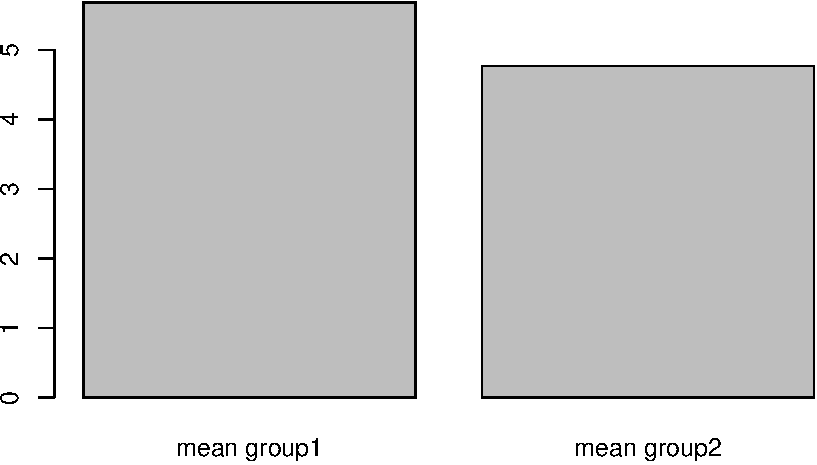
\includegraphics{intro_to_stats_files/figure-latex/unnamed-chunk-4-1.pdf}

Imagine drawing a line between the tops of the bars, like this:

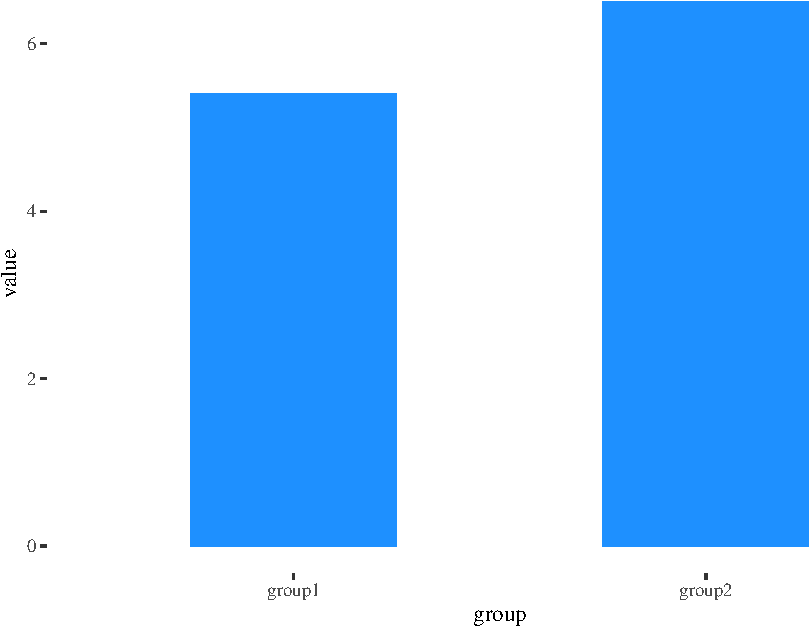
\includegraphics{intro_to_stats_files/figure-latex/unnamed-chunk-5-1.pdf}

The slope of that line tells us about the difference in the means. If it is flat no difference, if it isnt flat maybe there is a difference.

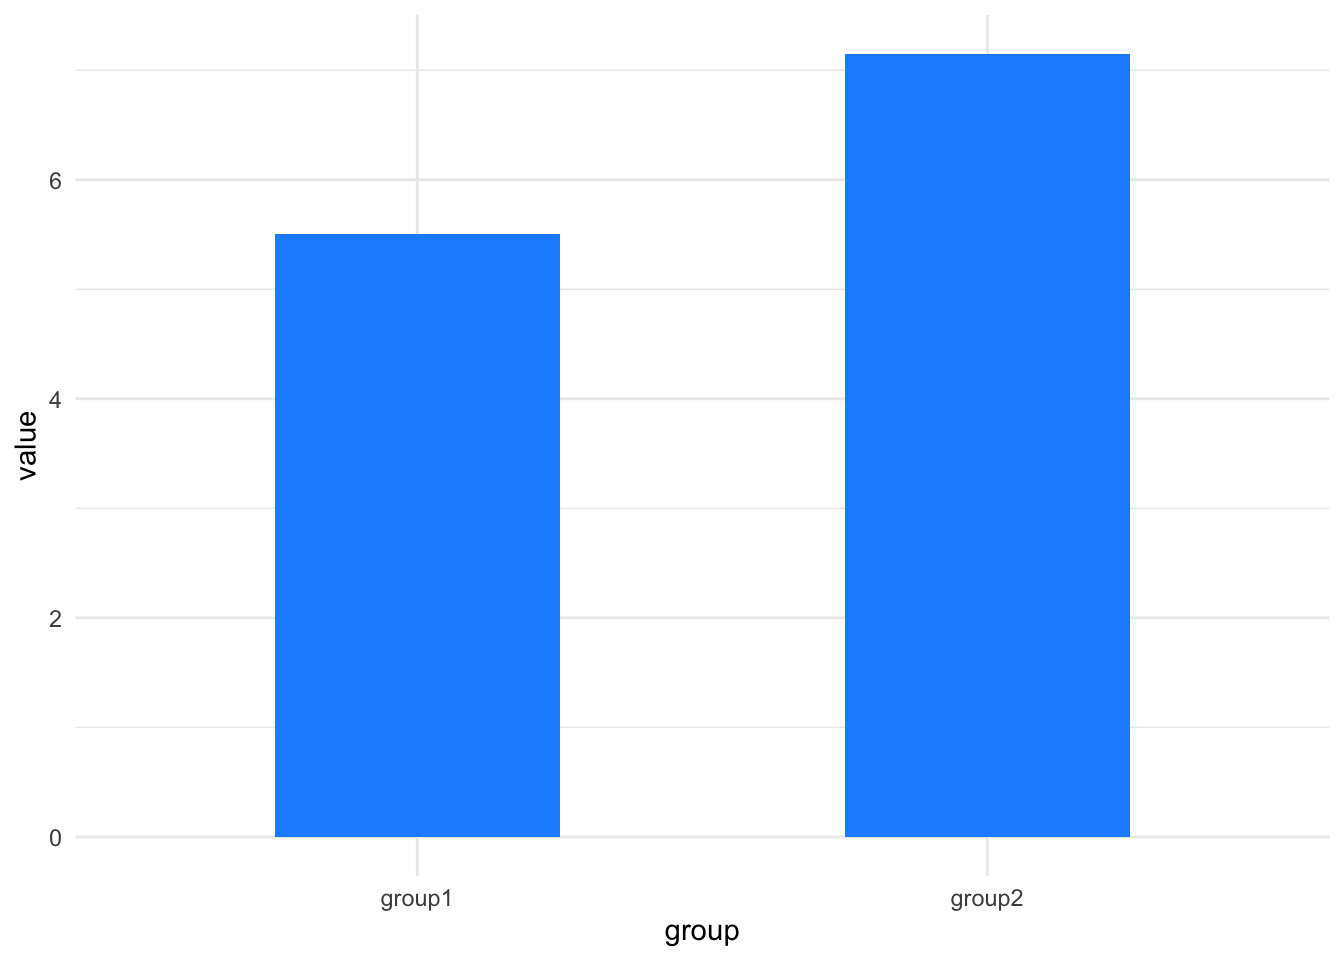
\includegraphics[width=0.5\linewidth]{intro_to_stats_files/figure-latex/unnamed-chunk-6-1} 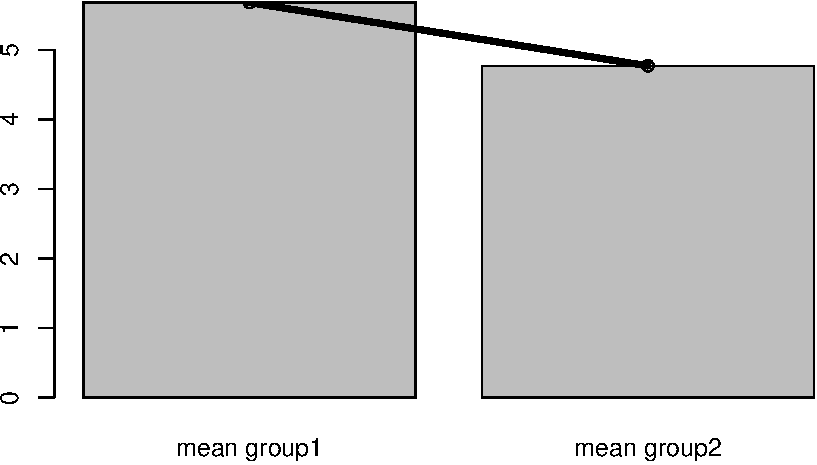
\includegraphics[width=0.5\linewidth]{intro_to_stats_files/figure-latex/unnamed-chunk-6-2}

And that is the logic we will be following in this little book. All we will do is learn to look for a slope of a line. We'll look at using a statistical tool called a linear model, which tries to create a straight line that matches the data, so is contains the equation of a straight line but elaborates on the equation alone by providing measures of believability about the slope and other things. The technique we will learn will give us a framework for thinking about performing hypothesis testing in all sorts of comparisons including \(t\)-tests, ANOVA etc and with elaborations we'll be able to see how to use the same framework for the other class of tests that we often use, the non-parametric tests.

\hypertarget{the-linear-model}{%
\chapter{The Linear Model}\label{the-linear-model}}

\hypertarget{straight-line-relationships-are-described-using-two-parameters}{%
\section{Straight line relationships are described using two parameters}\label{straight-line-relationships-are-described-using-two-parameters}}

Its all about \(y = ax + b\) (or \(y = mx + c\), depending on where you went to school). These two equivalent formulae are the standard high-school equations for describing a straight line. They represent how the quantity \(y\) changes as \(x\) does.

As a refresher, \(a\) tells us how much \(y\) increases for every unit increase in \(x\). Here's an example for the equation \(y = 4x\)

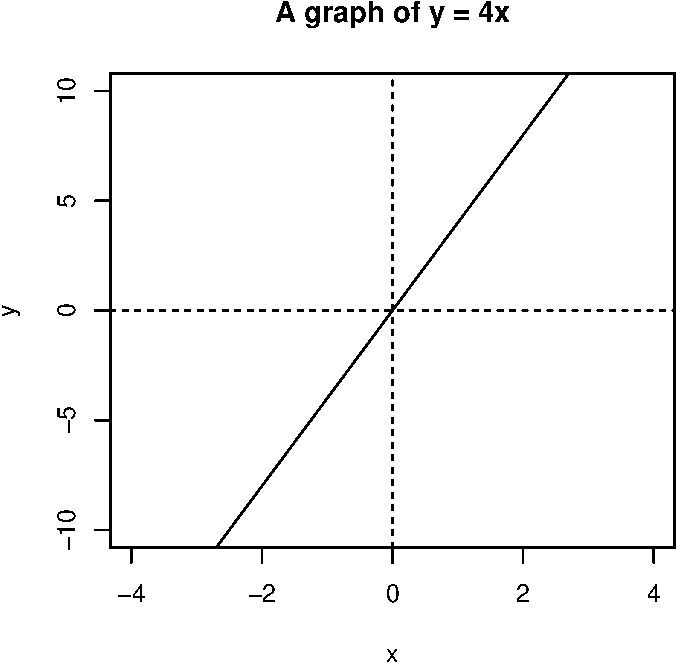
\includegraphics{intro_to_stats_files/figure-latex/unnamed-chunk-7-1.pdf}

If we play about with that value, the slope of the line changes, the \(b\) term is known as the slope, or gradient, or more often because it is just a multiplier of \(x\) its called the coefficient. Here's some different coefficients just to prove that point

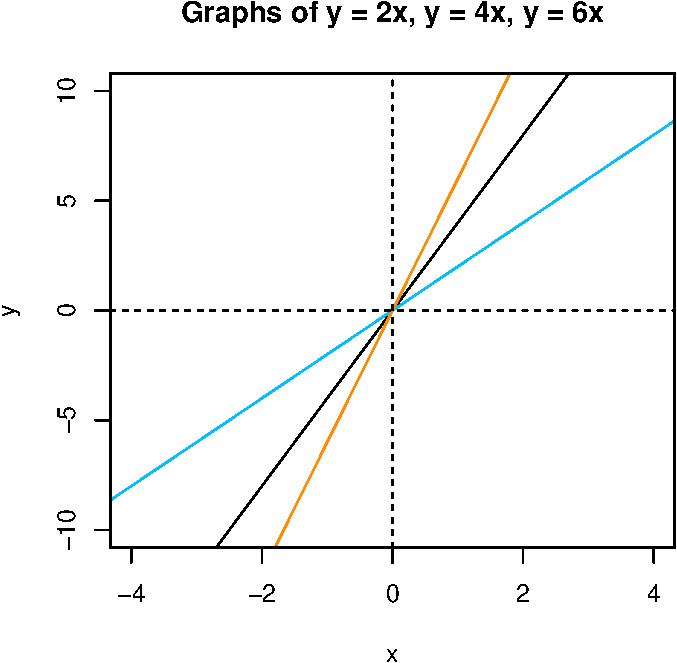
\includegraphics{intro_to_stats_files/figure-latex/unnamed-chunk-8-1.pdf}

The \(b\) part of the formula just tells us how much we add on to \(y\) after we've calculated the coefficient effect. It has the effect of pushing the line up and down the y-axis. When we look at the value of \(y\) for \(x = 0\) we get the position that the graph hits the y-axis so this number is often called the intercept. Here's a set of lines to show that.

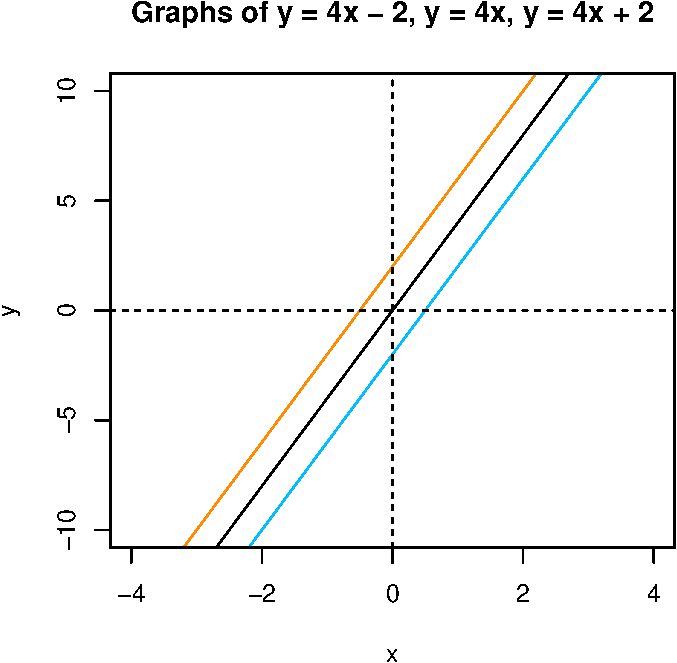
\includegraphics{intro_to_stats_files/figure-latex/unnamed-chunk-9-1.pdf}

That's all we need to know about the equation of the straight line. Now we need to look at how they're a useful tool when analysing experimental data.

TODO: TASK

\hypertarget{linear-models-try-to-create-a-linear-equation-from-data}{%
\section{Linear models try to create a linear equation from data}\label{linear-models-try-to-create-a-linear-equation-from-data}}

In this section we'll discuss what a linear model is, and how it is different yet related to the equation we've introduced above.

A linear model is a simplification of the relationship between some sets of numbers (in the simple case we will introduce here, it is two sets, but it can be more). At its heart is a straight line, with the equation we discussed above and a certain set of values for \(a\), the coefficient and \(b\), the intercept and some other statistics that describe the strength of the relationship.

Let's walk through building one, graphically and in R.

First we need some sets of values, \(x\) and \(y\). Usually, these would be from an experiment, but here I'll make some toy ones.

\begin{Shaded}
\begin{Highlighting}[]
\KeywordTok{set.seed}\NormalTok{(}\StringTok{"456"}\NormalTok{)}
\NormalTok{x <-}\StringTok{ }\KeywordTok{runif}\NormalTok{(}\DecValTok{20}\NormalTok{, }\DecValTok{5}\NormalTok{, }\DecValTok{15}\NormalTok{)}
\NormalTok{y <-}\StringTok{ }\NormalTok{x }\OperatorTok{*}\StringTok{ }\DecValTok{2} \OperatorTok{+}\StringTok{ }\KeywordTok{rnorm}\NormalTok{(}\DecValTok{20}\NormalTok{)}
\KeywordTok{plot}\NormalTok{(x,y)}
\end{Highlighting}
\end{Shaded}

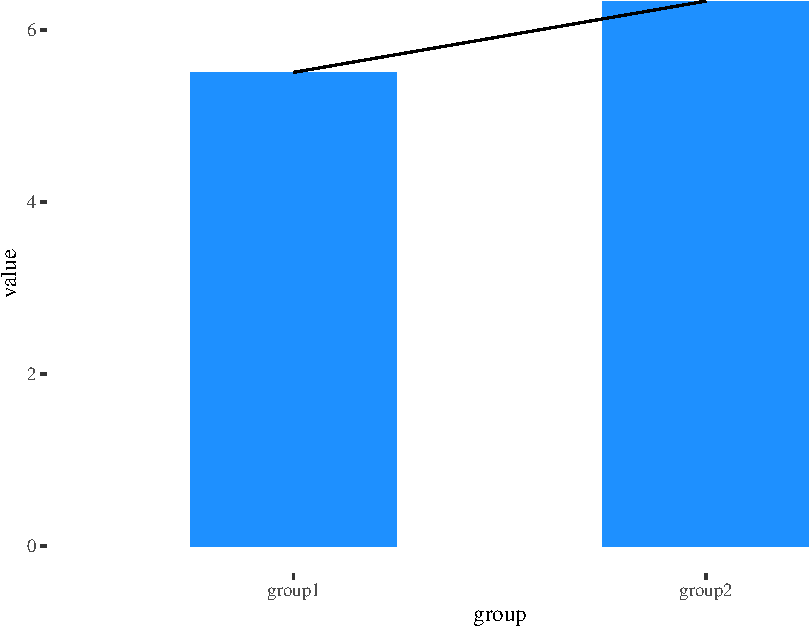
\includegraphics{intro_to_stats_files/figure-latex/unnamed-chunk-10-1.pdf}

The graph shows 20 random \(x\) values between 5 and 15 plotted against 20 \(y\) values which are calculated as \(2x\) with a little random noise added. We can see that there is definitely a relationship (not least because we engineered it that way). The objective of the linear model is to quantify and describe the relationship in some way. Here's where the linear equation comes in, if we could come up with a line that fitted through the data we could use the linear equation of that line to roughly describe - or model - our data. Skipping to the chase there is absolutely a way to get the line from the data. The methods are described in lots of statistics books so I won't repeat them, but you may be familiar with the general methods, its the `line of best fit' according to the ordinary least squares method. The function we need in R is \texttt{lm()} and it works like this

\begin{Shaded}
\begin{Highlighting}[]
\KeywordTok{lm}\NormalTok{(y }\OperatorTok{~}\StringTok{ }\NormalTok{x)}
\end{Highlighting}
\end{Shaded}

Thats it! The function \texttt{lm()} does the work, it takes a fairly odd syntax, though. The \texttt{y\ \textasciitilde{}\ x} bit is an R formula and describes the relationship you want to examine, you can read it as \texttt{y\ depends\ on\ x}. The \texttt{y} and \texttt{x} we're referring to here are the two vectors of numbers we created and plotted above.

Looking at the function output we get this

\begin{verbatim}
## 
## Call:
## lm(formula = y ~ x)
## 
## Coefficients:
## (Intercept)            x  
##       0.778        1.955
\end{verbatim}

These are the intercept (\(b\)) and the coefficient of \(x\) (\(a\)) that we need to describe the line. So our data are described by the line \(y = 1.955x + 0.778\).

So this line is a model of the data, it's a model in the sense that it is something that represents our data, but isn't it. The line alone can be useful to teach us about our data, but there's more to the linear model than just the line.

\hypertarget{linear-models-describe-relationships-between-variables}{%
\section{Linear models describe relationships between variables}\label{linear-models-describe-relationships-between-variables}}

Beyond working out the equation of the line, the linear model process aims to quantify and describe relationships between the variables in the data, in our toy example the variables are \(x\) and \(y\). Specifically when we say `relationship', we mean whether a change in the value of \(x\) appears to go along with some change in the value of \(y\).

In other words, we can think of relationship as being the slope. If \(x\) causes some change in \(y\) when we plot it then there must be a slope. We call the slope \(a\) in our equation of a line and we call it the coefficient of the \(x\) term in our linear model. These are all equivalent interpretations for our purposes, slope, relationship, coefficient and \(a\) just mean that \$

Linear models calculate statistics to help us decide whether the coefficient/slope/\(a\) of the relationship we observe is important or not.

\hypertarget{not-all-lines-of-best-fit-are-equally-good}{%
\section{Not all lines of best fit are equally good}\label{not-all-lines-of-best-fit-are-equally-good}}

Although a line of best fit can always be calculated, the line might not be worth much. Consider two sets of very similar numbers. Here's two vectors of random numbers with the same mean and their plot.

\begin{Shaded}
\begin{Highlighting}[]
\NormalTok{x1 <-}\StringTok{ }\KeywordTok{runif}\NormalTok{(}\DecValTok{20}\NormalTok{, }\DecValTok{5}\NormalTok{, }\DecValTok{15}\NormalTok{)}
\NormalTok{y1 <-}\StringTok{ }\KeywordTok{runif}\NormalTok{(}\DecValTok{20}\NormalTok{, }\DecValTok{5}\NormalTok{, }\DecValTok{15}\NormalTok{)}

\KeywordTok{plot}\NormalTok{(x1, y1)}
\end{Highlighting}
\end{Shaded}

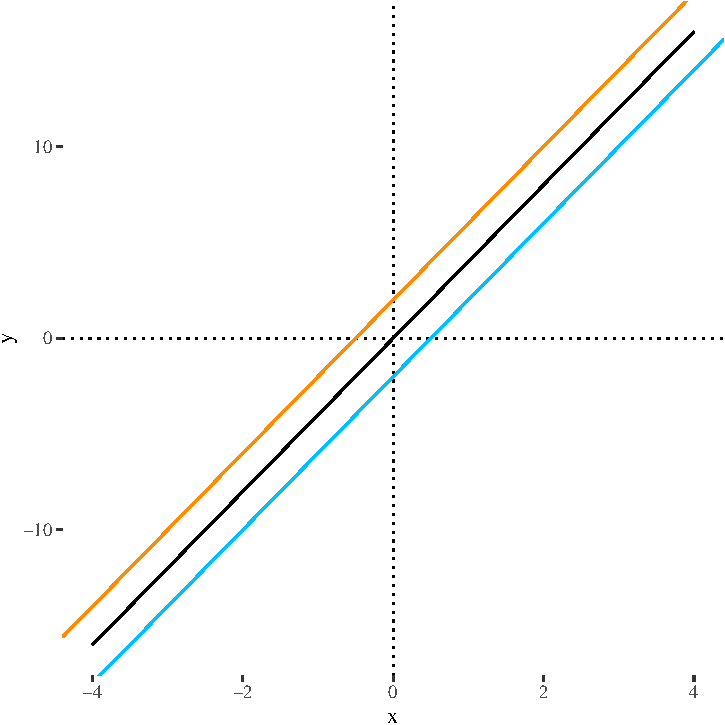
\includegraphics{intro_to_stats_files/figure-latex/unnamed-chunk-13-1.pdf}

We can definitely calculate a line that fits these,

\begin{Shaded}
\begin{Highlighting}[]
\KeywordTok{lm}\NormalTok{(y1 }\OperatorTok{~}\StringTok{ }\NormalTok{x1)}
\end{Highlighting}
\end{Shaded}

\begin{verbatim}
## 
## Call:
## lm(formula = y1 ~ x1)
## 
## Coefficients:
## (Intercept)           x1  
##     10.4695       0.1103
\end{verbatim}

and it would be \(y = 0.1103x + 10.6495\). But if we compare the fit of those lines, like in these plots

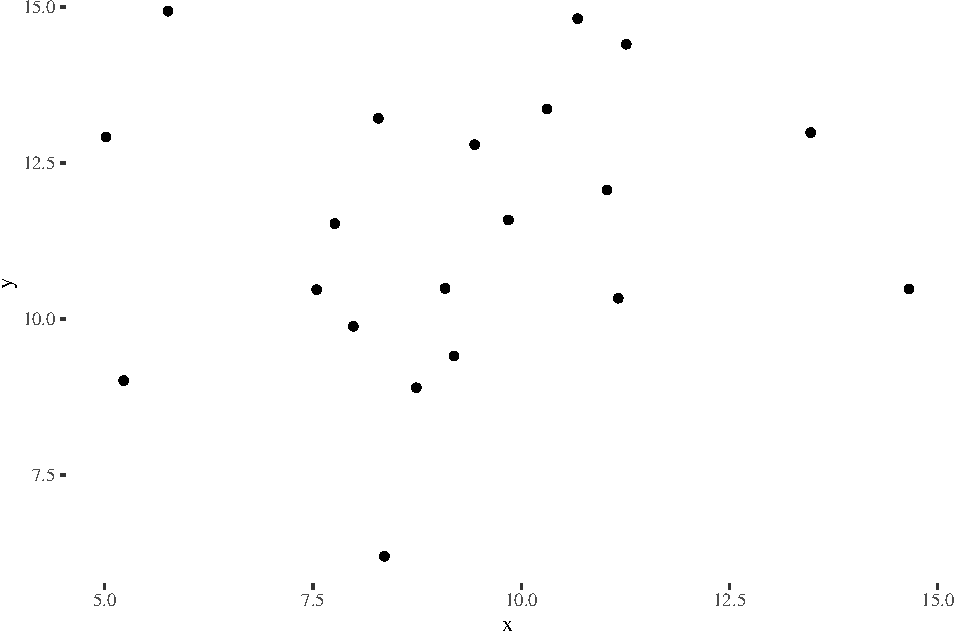
\includegraphics[width=0.5\linewidth]{intro_to_stats_files/figure-latex/unnamed-chunk-15-1} 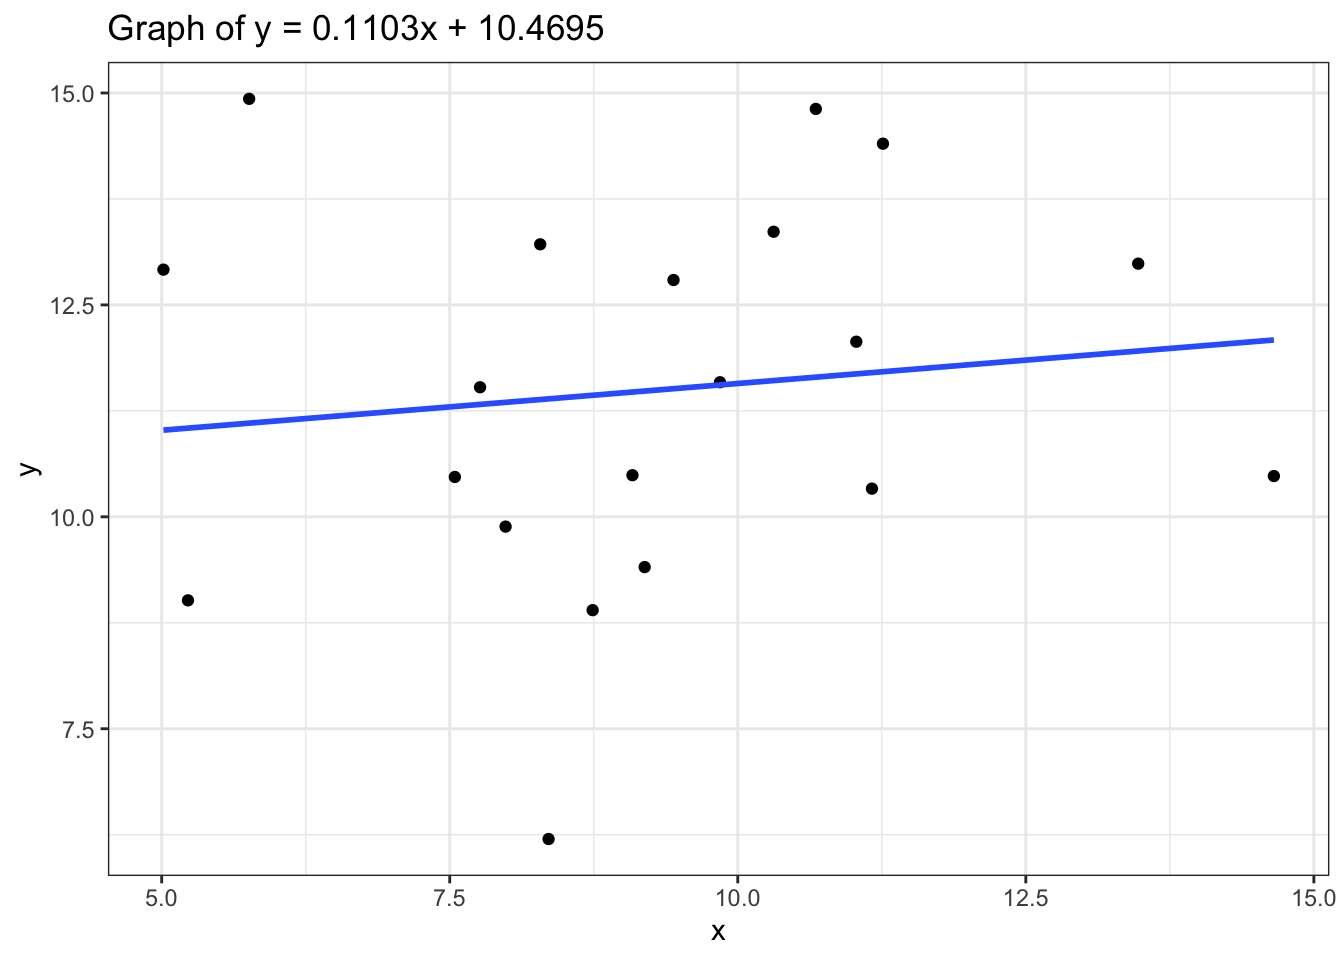
\includegraphics[width=0.5\linewidth]{intro_to_stats_files/figure-latex/unnamed-chunk-15-2}

we can clearly see that not all lines are created equal. The first line fits the data much more closely than the second one. We can also see that the relationship between \(x\) and \(y\) is much weaker in the second set than in the first (the coefficient/slope/\(a\) is weaker. So a sensible linear model of our data would give us not just the equation but also measures of the believability of the line.

\hypertarget{linear-models-contain-statistics-describing-the-goodness-of-the-model}{%
\section{Linear models contain statistics describing the goodness of the model}\label{linear-models-contain-statistics-describing-the-goodness-of-the-model}}

The same function we've already used - \texttt{lm()} - calculates certain statisitics. We can print them using the \texttt{summary()} function.

\begin{Shaded}
\begin{Highlighting}[]
\NormalTok{model <-}\StringTok{ }\KeywordTok{lm}\NormalTok{(y }\OperatorTok{~}\StringTok{ }\NormalTok{x)}
\KeywordTok{summary}\NormalTok{(model)}
\end{Highlighting}
\end{Shaded}

\begin{verbatim}
## 
## Call:
## lm(formula = y ~ x)
## 
## Residuals:
##      Min       1Q   Median       3Q      Max 
## -2.17560 -1.00570 -0.01092  1.17016  1.83047 
## 
## Coefficients:
##             Estimate Std. Error t value Pr(>|t|)    
## (Intercept)   0.7780     1.1442    0.68    0.505    
## x             1.9555     0.1122   17.42 1.03e-12 ***
## ---
## Signif. codes:  0 '***' 0.001 '**' 0.01 '*' 0.05 '.' 0.1 ' ' 1
## 
## Residual standard error: 1.303 on 18 degrees of freedom
## Multiple R-squared:  0.944,  Adjusted R-squared:  0.9409 
## F-statistic: 303.6 on 1 and 18 DF,  p-value: 1.027e-12
\end{verbatim}

This output is verbose, there are four blocks.

\begin{enumerate}
\def\labelenumi{\arabic{enumi}.}
\tightlist
\item
  \texttt{Model\ Call} - just a restatment of the function we called
\item
  \texttt{Residuals} - a set of measures of the distribution of the residuals, we don't worry about this yet.
\item
  \texttt{Coefficients} - the terms of the equation and their statistics; so the intercept (\(b\)) and the coefficient of \texttt{x} (\(a\)) that we've already seen and the \texttt{Estimate} (computed values of those). We see also columns of statistics for each.
\item
  The model level statistics summary - some statistics that apply to the whole model.
\end{enumerate}

Let's start at the bottom and look at model level summary.

\hypertarget{residual-standard-error}{%
\subsection{Residual Standard Error}\label{residual-standard-error}}

This is the measure of how well the line fits the data. Unlike the linear equation, the linear model has an extra error term, \(e\) which represents the average distance from the actual measurments to the line in the y-axis. So in a linear model we have a formula that looks like this

\begin{equation}
 y = ax + b + e
\end{equation}

The \(e\) term adds something onto the y value of the whole equation; the more we need to add on to the value of the \(x\) from the line to get the real \(y\). Logically, the bigger \(e\) is the more the error in the model overall.

If you look at the plots again with those distance drawn in you can see quite clearly the residual error for the second model is much bigger than for the first.

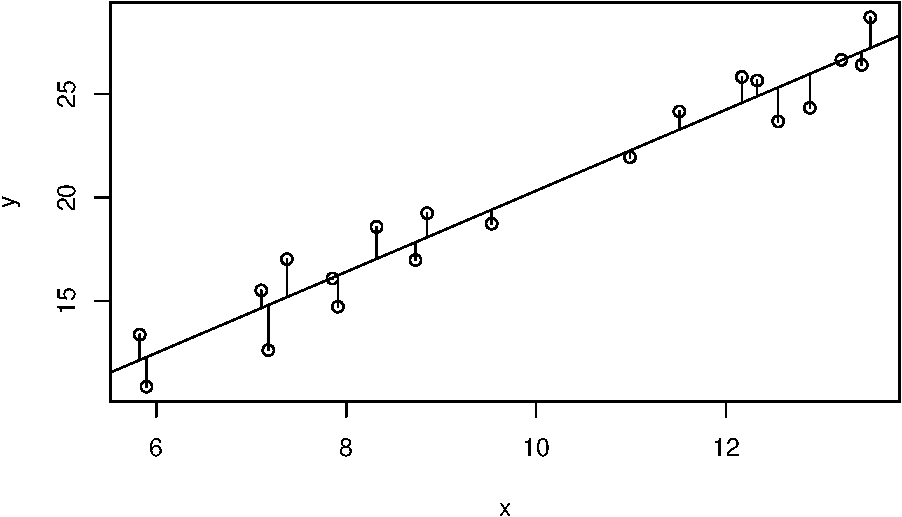
\includegraphics[width=0.5\linewidth]{intro_to_stats_files/figure-latex/unnamed-chunk-17-1} 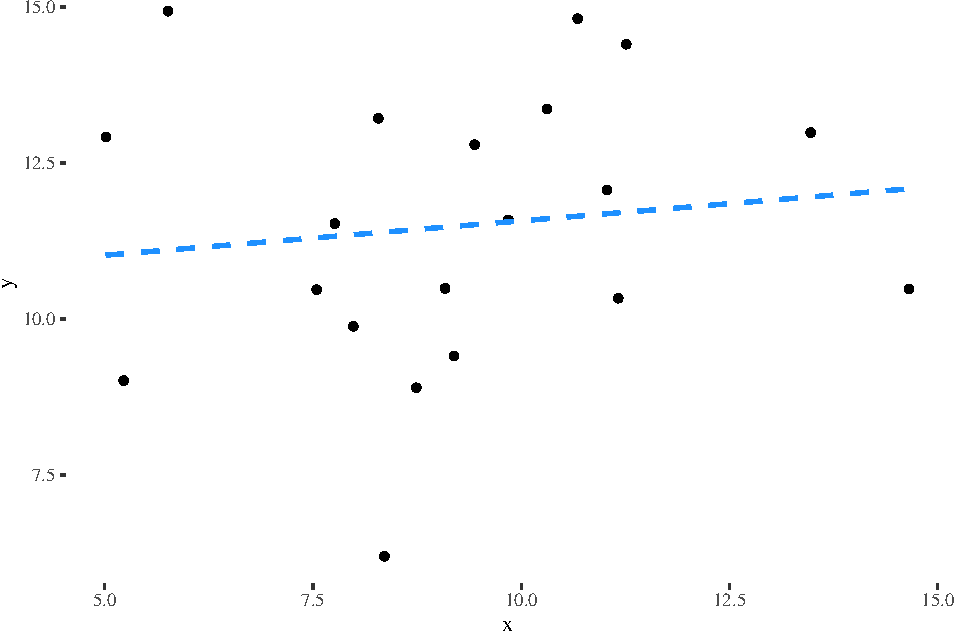
\includegraphics[width=0.5\linewidth]{intro_to_stats_files/figure-latex/unnamed-chunk-17-2}

\hypertarget{r2}{%
\subsection{\texorpdfstring{\(R^2\)}{R\^{}2}}\label{r2}}

\(R^2\) is a measure of how well the model fits the data. If you're thinking correlation coefficient here, then you're in the right area. \(R^2\) describes the proportion of variance in the \(y\) values that can be explained by the \(x\) values. The \(R^2\) always falls between 0 and 1. Closer to 1 is usually better, but it is very domain and dataset dependent. With small and biological data sets, we don't always see values close to that because of the noise of the system.

The proper one to use in most cases is the \texttt{Adjusted\ R-squared}.

\hypertarget{r2-versus-residual-standard-error}{%
\subsection{\texorpdfstring{\(R^2\) versus Residual Standard Error}{R\^{}2 versus Residual Standard Error}}\label{r2-versus-residual-standard-error}}

So what's the difference between these two - at first glance they do the same thing. The major difference is that RSE is in the units of the data and \(R^2\) is in relative units, so you can use them in different situations e.g if you want to make your model work within particular tolerances or you want to compare models in different units.

\hypertarget{f-statistic}{%
\subsection{\texorpdfstring{\(F\)-Statistic}{F-Statistic}}\label{f-statistic}}

The \(F\)-Statistic is an indicator of a relationship between the \(x\) and \(y\) values of the model. In effect its testing how much better the relationship is in your model relative to a model in which the relationship is completely random. When the \(F\)-statistic is at 1, the relationship is no stronger than a random relationship. The further above 1 this value is, the more it is likely there is a real relationship in the model. The \(p\) value here is the \(p\) that this size of \(F\) would occur in a random relationship with a similar dataset size. As with the other statistics, the size of \(F\) is dependent on the domain and data being analysed.

\hypertarget{coefficients-have-statistics}{%
\section{Coefficients have statistics}\label{coefficients-have-statistics}}

Along with these model level statistics, linear modelling with \texttt{lm()} gives us a set of statistics \emph{per coefficient}. These measure the effect that each coefficient has.

\hypertarget{estimate}{%
\subsection{Estimate}\label{estimate}}

These are the \texttt{Estimate}, which is the actual value of the coefficient from the model. We will see that along with Intercept we can have models with more than one other coefficient. These are given in the units of the data.

\hypertarget{std.-error}{%
\subsection{Std. Error}\label{std.-error}}

A measure of the variability of the strength of the effect, so if some \(x\) points give more pronounced \(y\) values at similar coefficient values, you get a higher variability of the strength. Generally lower standard error of the coefficient is good.

\hypertarget{t-value}{%
\subsection{\texorpdfstring{\(t\)-value}{t-value}}\label{t-value}}

An estimate of how extreme the coefficient value is, basically how many Standard Deviations away the estimate is from the centre of a presumed normal distribution with mean 0. It is absolutely a \(t\)-test \(t\)-value, and like in a \(t\)-test we want it to be high. The higher \(t\) is, then the more likely that the coefficient is not at 0.

\hypertarget{wait-what}{%
\subsubsection{Wait, what?}\label{wait-what}}

Why would we care whether the coefficient is at 0 or not? Well, because if it is 0, then it's having no effect on the model. Consider again the equation of a line

\begin{equation}
y = ax + b
\end{equation}

If we let the coefficient \(a = 0\), this happens

\begin{equation}
y = 0 x + b\\
y = b
\end{equation}

The coefficient disappears, its having no effect!

If the coefficient is not many standard deviations away from 0, its probably not having much effect on the relationship. The \(t\) value tries to work out whether, given the data, the coefficient is in anyway different to 0.

In English, we are really saying that the size if the slope is not likely to be 0. That it is not likely that there is no relationship. Which is weak inference, but is \emph{exactly} the same sort of inference that all the other hypothesis test make and is exactly the same interpretation

\textbf{pull\_out}
A lot of researchers get the impression that \(t\)-tests, ANOVAs and other hypothesis tests tell you whether something is signifcant with probability \(p\). This is a massive misinterpretation. They do no such thing.

In fact what a hypothesis test tells you is how often you'd see this difference between two means of some numbers if the real difference was 0.

This is resolutely not the same as saying they are definitely different. Just that they're not likely to be the same as 0. The \(p\) in \(p\) value is usually taken to mean probability, but if it stands for anything it should be `probably not 0'.

Hypothesis testing like this has been criticised for being weak inference, and not without reason.

\textbf{pull\_out}

Of course, this will depend on the size of the standard deviation. The noisier the data or the smaller the sample size then the larger this value will need to be to be important.

\hypertarget{prt}{%
\subsection{\texorpdfstring{\(Pr(>|t|)\)}{Pr(\textgreater{}\textbar{}t\textbar{})}}\label{prt}}

This weird shorthand expression is just giving the probability of getting a value larger than the \(t\)-value. This comes from a \(t\)-test within the model and takes into account the dataset size and variability, you can think of it as the \(p\)-value of a test asking whether the coefficient is equal to 0. So if \(p\) is less than 0.05 you can say that the value of the coefficient is not likely to be 0 and therefore is having an effect on the model.

\hypertarget{a-non-zero-slope-is-what-matters}{%
\section{A non-zero slope is what matters}\label{a-non-zero-slope-is-what-matters}}

By looking at the \(p\)-value of the coefficient then, we can see whether there is a significant relationship or, more accurately a non-zero slope

We can really emphasise by looking at the plots of lines we looked at earlier.

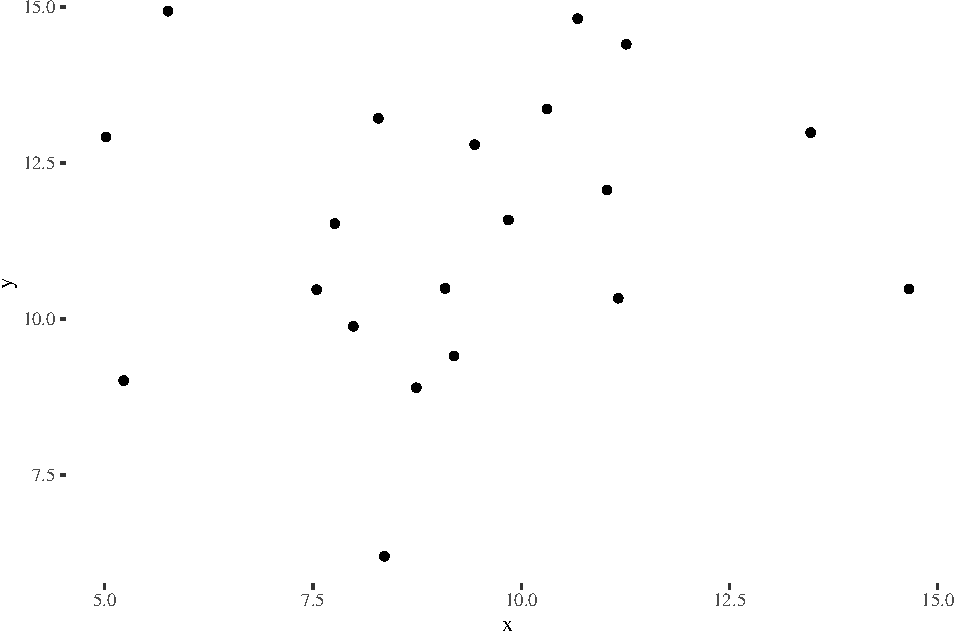
\includegraphics[width=0.5\linewidth]{intro_to_stats_files/figure-latex/unnamed-chunk-18-1} 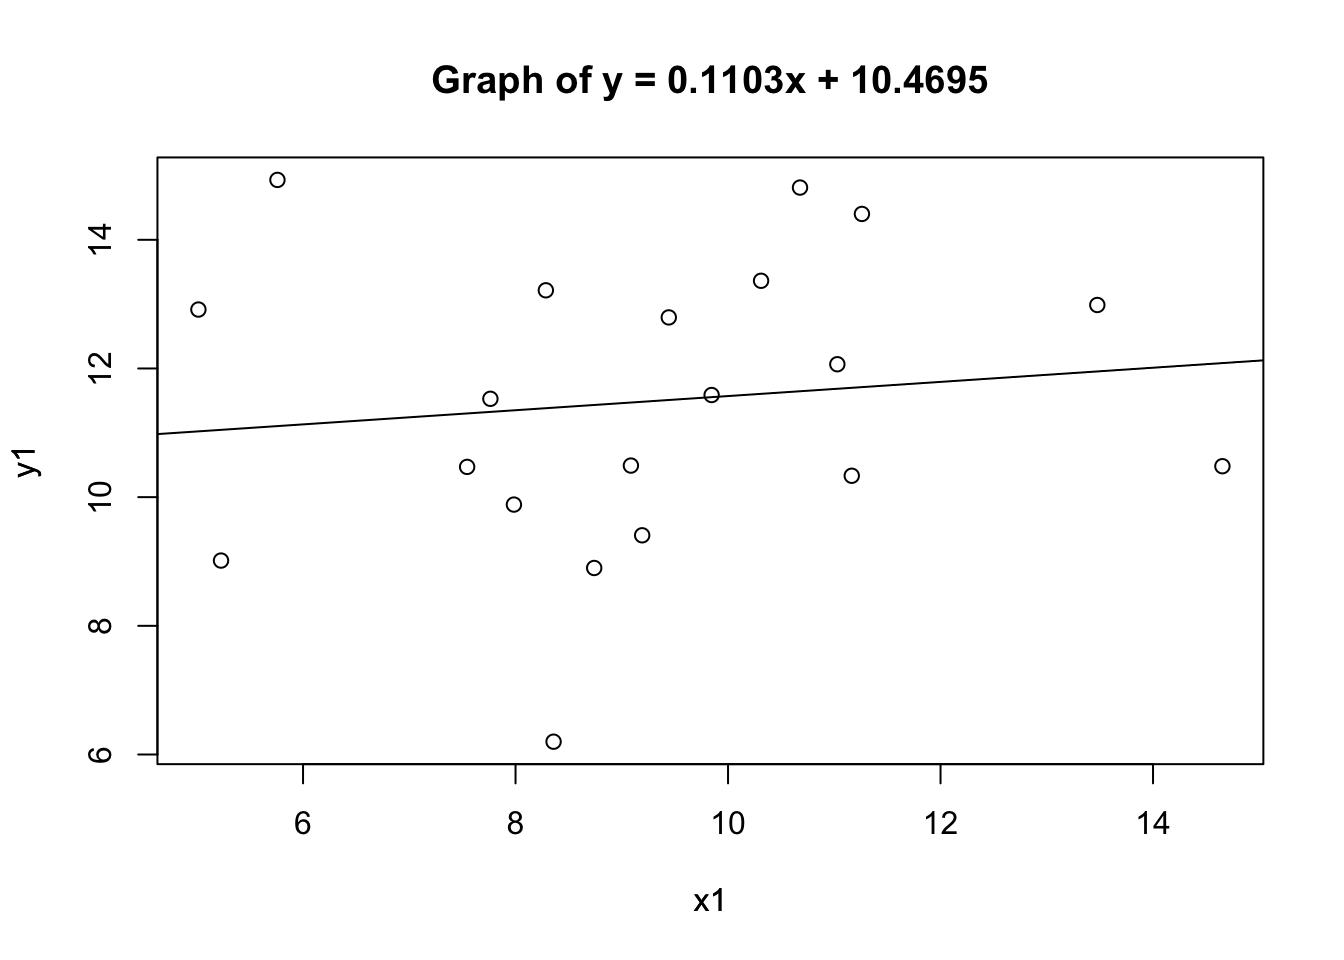
\includegraphics[width=0.5\linewidth]{intro_to_stats_files/figure-latex/unnamed-chunk-18-2}

The slope of the second plot is weaker, it's much flatter - much closer to zero, in fact given the spread of the data we aren't that confident that it isn't a flat (zero) slope, so we aren't that confident that there is a significant relationship.

It is this feature that will help us in our overall goal of using the linear model in doing the work of all the other statistical tests we commonly use. If we have a good model and a good fit, then we can make really flexible use of the slope by looking at the significance of the coefficient.

\hypertarget{major-points}{%
\section{Major points}\label{major-points}}

After all that inspection of the linear model, here's what you need to remember:

\begin{enumerate}
\def\labelenumi{\arabic{enumi}.}
\tightlist
\item
  Linear models describe relationships between sets of numbers (variables)
\item
  The creation of the model generates statistics about the goodness of the model
\item
  A non-zero coefficient (slope) means there is not likely to be no relationship (!)
\end{enumerate}

\begin{center}\rule{0.5\linewidth}{0.5pt}\end{center}

Pretty soon, someone would've made some complaint about variability and that we should demonstrate the extent of that, something we might've done with error bars, and then someone like me would come along and say that even that isn't optimal so you'd better use dots, like this:

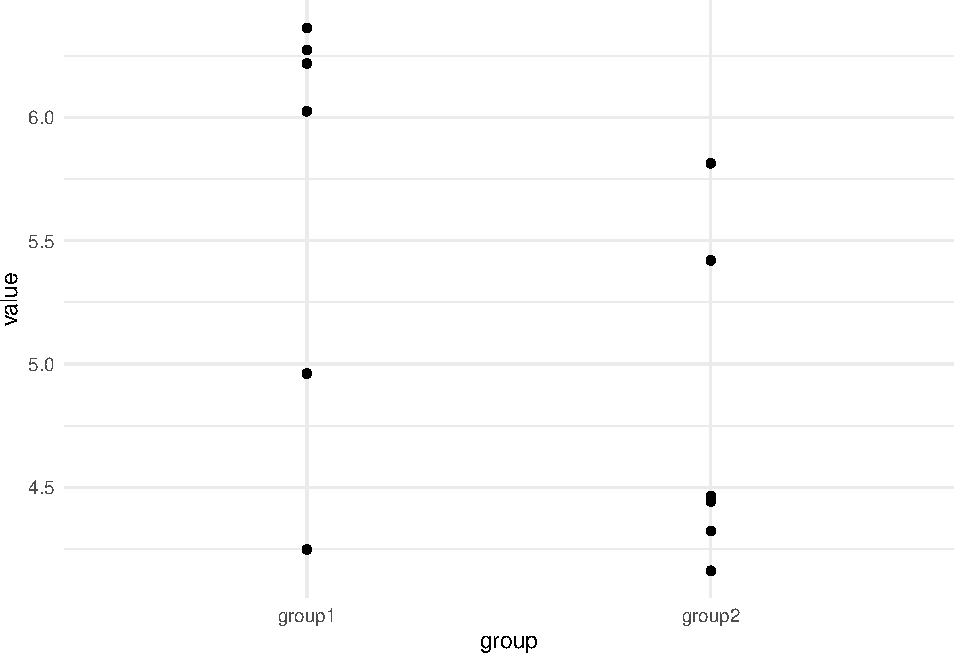
\includegraphics{intro_to_stats_files/figure-latex/unnamed-chunk-19-1.pdf}

\hypertarget{t-tests-and-linear-models}{%
\chapter{\texorpdfstring{\(t\)-tests and linear models}{t-tests and linear models}}\label{t-tests-and-linear-models}}

In this section we'll look at how the linear model can be used as a conceptual tool to understand the sort of comparison a \(t\)-test does and as a straightforward way to perform a hypothesis test.

\hypertarget{recap}{%
\section{Recap}\label{recap}}

Because I like hammering this point home, Im going to recap two important points from our work on linear models.

\begin{enumerate}
\def\labelenumi{\arabic{enumi}.}
\tightlist
\item
  The slope of the model is the important thing
\item
  `Significance' tests only test whether the difference between two things is `probably not 0'
\end{enumerate}

\hypertarget{the-slope-of-the-model-again}{%
\subsection{The slope of the model again}\label{the-slope-of-the-model-again}}

Recall the linear model equation

\begin{equation}
y = ax + b
\end{equation}

and that if we let the coefficient \(a = 0\), the effect of \(x\) disappears

\begin{equation}
y = 0 x + b\\
y = b
\end{equation}

So the logical conclusion is that if we have a coefficient that is non-zero, we have a relationship/effect of \(x\) on \(y\).

It is this property that let's us use the linear model to work out whether there is a significant difference between groups! That is to say we can use it as a \(t\)-test.

However, the second we try to apply what we've learned with the linear model to a two-sample dataset we hit an apparent problem because we've learned how to make linear models from datasets with a continuous, numeric \(x\)-axis, but the data we have for a \(t\)-test has a very different two category look, something like these here:

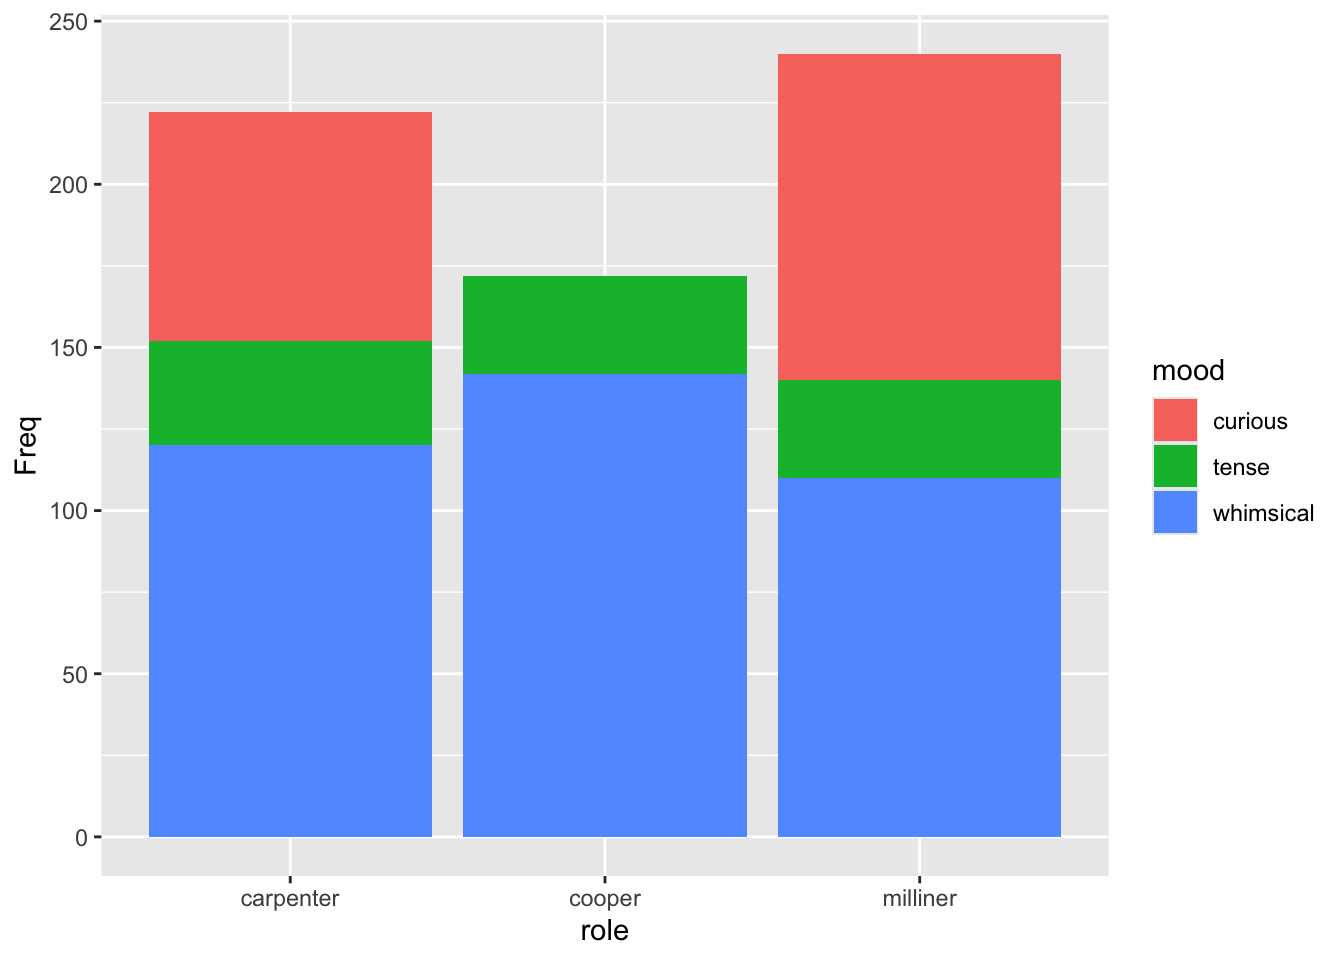
\includegraphics[width=0.5\linewidth]{intro_to_stats_files/figure-latex/unnamed-chunk-20-1} 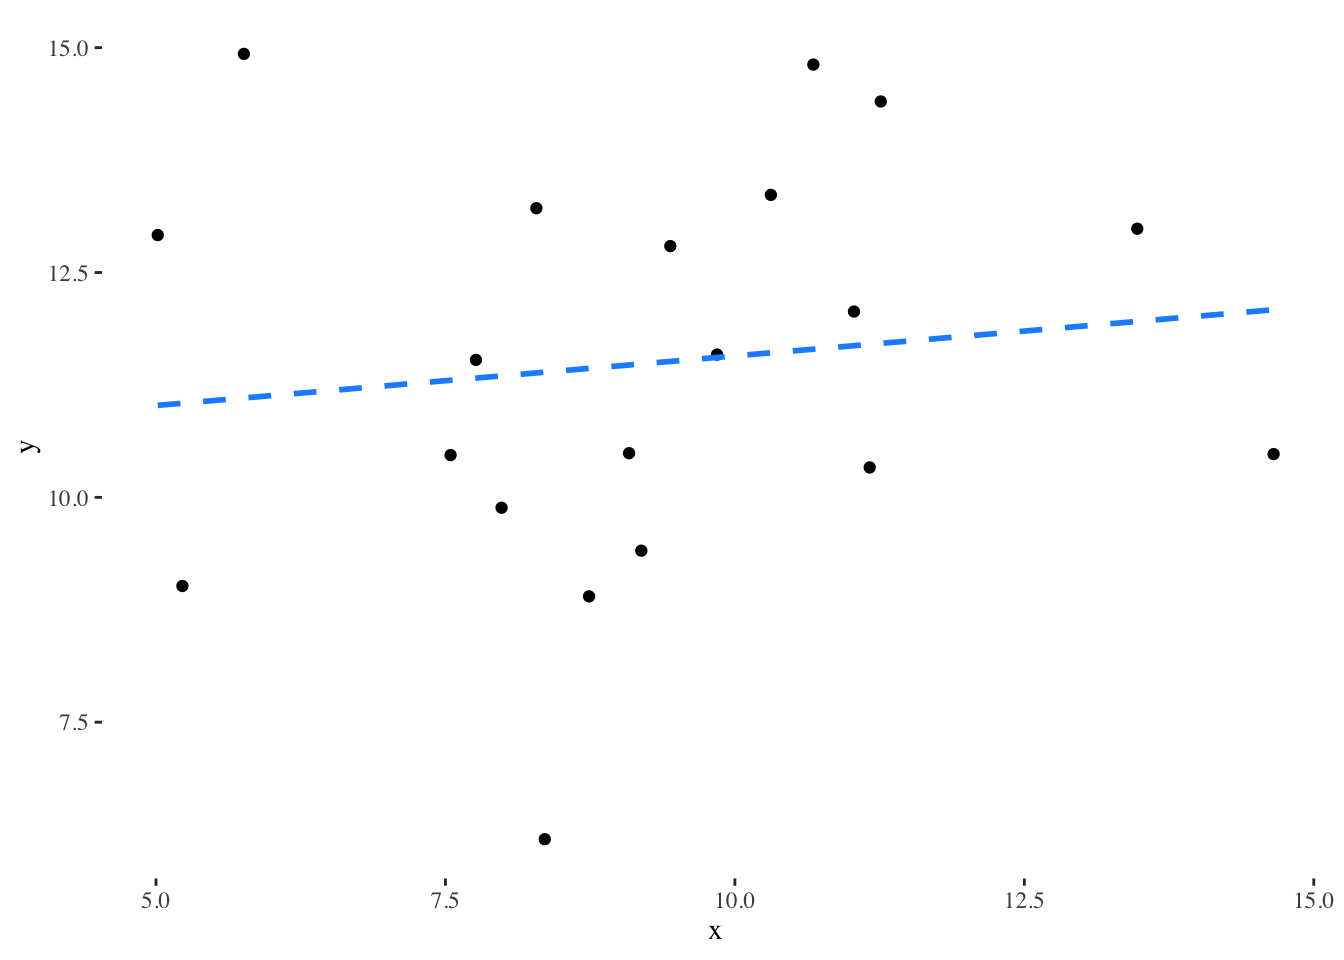
\includegraphics[width=0.5\linewidth]{intro_to_stats_files/figure-latex/unnamed-chunk-20-2}

The question then is what do we do with the categoric data to put it in a linear model?

The first step is to realise that although we are used to thinking of the each of the bars representing a single number, that single number is (almost always) a mean of replicate values, so we go back to those source numbers as a first step

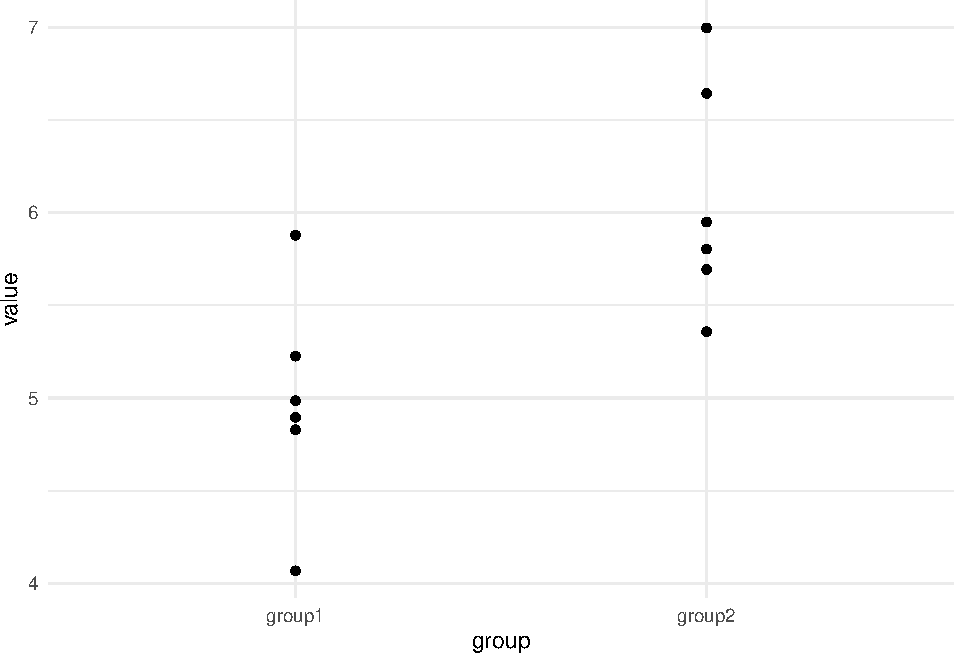
\includegraphics{intro_to_stats_files/figure-latex/unnamed-chunk-21-1.pdf}

and we have something a lot more like the scatterplot we're used to. The next step is to replace the categories with numbers for the \(x\)-axis. That means going from data like this

\begin{tabular}{r|r}
\hline
group1 & group2\\
\hline
4.895422 & 5.949330\\
\hline
5.225740 & 5.357527\\
\hline
4.828976 & 5.803222\\
\hline
5.878021 & 5.693268\\
\hline
4.068426 & 6.995864\\
\hline
4.985580 & 6.642633\\
\hline
\end{tabular}

to this

\begin{tabular}{l|r|r}
\hline
group & value & x\\
\hline
group1 & 4.895422 & 0\\
\hline
group1 & 5.225740 & 0\\
\hline
group1 & 4.828976 & 0\\
\hline
group1 & 5.878021 & 0\\
\hline
group1 & 4.068426 & 0\\
\hline
group1 & 4.985580 & 0\\
\hline
group2 & 5.949330 & 1\\
\hline
group2 & 5.357527 & 1\\
\hline
group2 & 5.803222 & 1\\
\hline
group2 & 5.693268 & 1\\
\hline
group2 & 6.995864 & 1\\
\hline
group2 & 6.642633 & 1\\
\hline
\end{tabular}

So now we can make a plot that looks a lot more like the one we're expecting

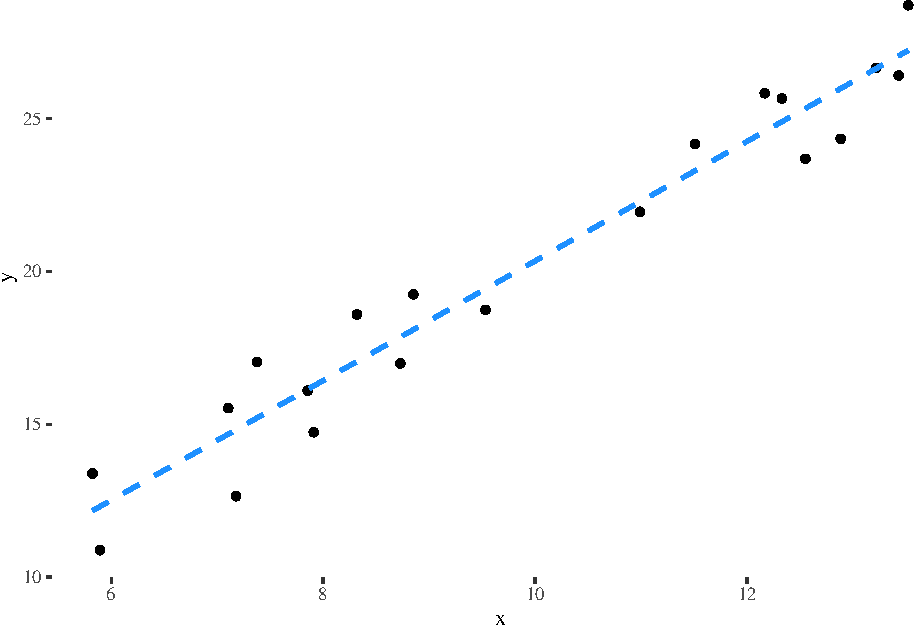
\includegraphics{intro_to_stats_files/figure-latex/unnamed-chunk-24-1.pdf}

albeit with the \(x\)-values in two places on the \(x\)-axis - its enough for us to make a slope on the line between the two groups and that means that we can use the linear model for the categoric data, as we did for the continuous.

If this seems like a bit of a `hack' then thats fair, but hacks are usually just pragmatic and useful solutions to problems, this one is completely mathematically legitimate as well as useful.

And if this change in the data reminds you of tidy data we've used in other courses, like dplyr, then that is no accident. Tidy data is designed to make this sort of analysis easy to work through, at least as far as organising the data goes.

The good news is that once we have our data setup, the \texttt{lm()} function just deals with these issues for us, we don't have to worry, the problem of contnuous or categoric \(x\)-axes just disappears!

So let's work through an example of a linear model based hypothesis test for differences between two groups that functions as a \(t\)-test.

\hypertarget{the-plantgrowth-data}{%
\section{The PlantGrowth data}\label{the-plantgrowth-data}}

R comes with lots of datasets built in. One if these is \texttt{PlantGrowth}, which describes the dry weight of plants in grams in replicated measurements in a control and two treatments. We can load it with \texttt{data()} and get a \texttt{summary()}

\begin{Shaded}
\begin{Highlighting}[]
\KeywordTok{data}\NormalTok{(}\StringTok{"PlantGrowth"}\NormalTok{)}
\KeywordTok{summary}\NormalTok{(PlantGrowth)}
\end{Highlighting}
\end{Shaded}

\begin{verbatim}
##      weight       group   
##  Min.   :3.590   ctrl:10  
##  1st Qu.:4.550   trt1:10  
##  Median :5.155   trt2:10  
##  Mean   :5.073            
##  3rd Qu.:5.530            
##  Max.   :6.310
\end{verbatim}

\begin{Shaded}
\begin{Highlighting}[]
\KeywordTok{head}\NormalTok{(PlantGrowth)}
\end{Highlighting}
\end{Shaded}

\begin{verbatim}
##   weight group
## 1   4.17  ctrl
## 2   5.58  ctrl
## 3   5.18  ctrl
## 4   6.11  ctrl
## 5   4.50  ctrl
## 6   4.61  ctrl
\end{verbatim}

We have three groups and one measurement, in our linear model this means that the \(x\) values would come from the \texttt{group} column - because it is categoric rather than continuous as we had before isn't a concern. The \(y\) values would come from the \texttt{weight} column.

In linear modelling jargon, the \(x\) values are called the independent or explanatory variable, simply because this is the one we changed over the course of the experiment. The \(y\) values are called the dependent or response variables as this is the one that responds or changes according to the changes in the independent variable.

For simplicity at this stage we'll work with two groups only. Let's remove \texttt{trt2}.

\begin{Shaded}
\begin{Highlighting}[]
\KeywordTok{library}\NormalTok{(dplyr)}
\NormalTok{two_groups <-}\StringTok{ }\NormalTok{PlantGrowth }\OperatorTok\StringTok{ }
\StringTok{  }\KeywordTok{filter}\NormalTok{(group }\OperatorTok{!=}\StringTok{ "trt2"}\NormalTok{) }\OperatorTok\StringTok{ }
\StringTok{  }\KeywordTok{droplevels}\NormalTok{()}

\KeywordTok{summary}\NormalTok{(two_groups)}
\end{Highlighting}
\end{Shaded}

\begin{verbatim}
##      weight       group   
##  Min.   :3.590   ctrl:10  
##  1st Qu.:4.388   trt1:10  
##  Median :4.750            
##  Mean   :4.846            
##  3rd Qu.:5.218            
##  Max.   :6.110
\end{verbatim}

With that done, we can look at the categorical scatter plot.

\begin{Shaded}
\begin{Highlighting}[]
\KeywordTok{library}\NormalTok{(ggplot2)}
\NormalTok{p <-}\StringTok{ }\KeywordTok{ggplot}\NormalTok{(two_groups) }\OperatorTok{+}\StringTok{ }
\StringTok{  }\KeywordTok{aes}\NormalTok{(group, weight) }\OperatorTok{+}\StringTok{ }
\StringTok{  }\KeywordTok{geom_point}\NormalTok{()}
\NormalTok{p}
\end{Highlighting}
\end{Shaded}

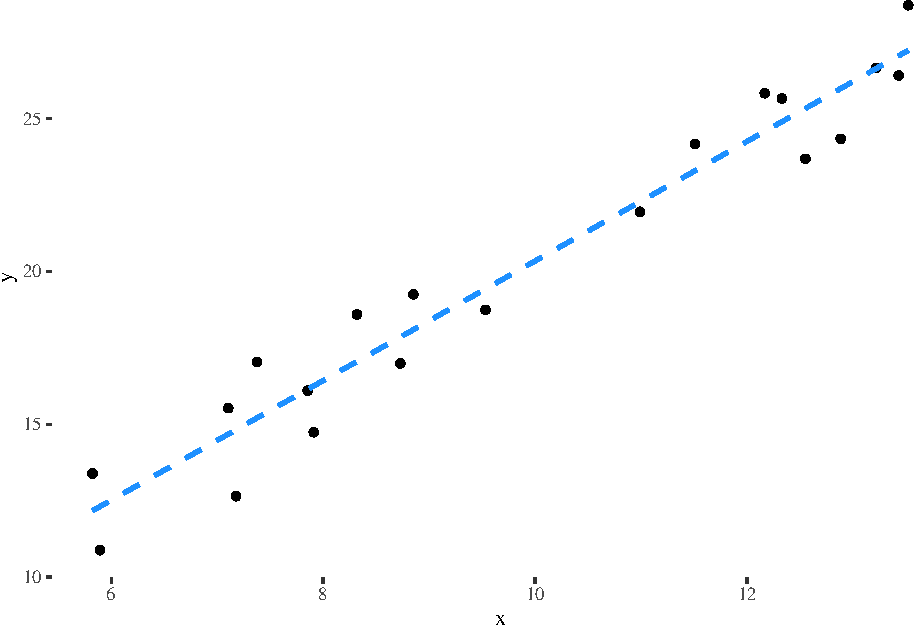
\includegraphics{intro_to_stats_files/figure-latex/unnamed-chunk-28-1.pdf}

We can clearly see the weight spread in each group. By eye we can see that the groups overlap in the \(y\)-axis (weight) quite considerably, though \texttt{trt1} seems to have a couple of data points that are lower.

\hypertarget{a-linear-model-with-a-categoric-x-axis}{%
\section{\texorpdfstring{A linear model with a categoric \(x\)-axis}{A linear model with a categoric x-axis}}\label{a-linear-model-with-a-categoric-x-axis}}

Let's make the linear model and get the intercept and coefficient of the line. This can be done with \texttt{lm()} as we did before, but because we have the data in a dataframe, we need to specify a \texttt{data} argument, which just means `look for the data in the given object'.

\begin{Shaded}
\begin{Highlighting}[]
\NormalTok{two_groups_model <-}\StringTok{ }\KeywordTok{lm}\NormalTok{(weight }\OperatorTok{~}\StringTok{ }\NormalTok{group, }\DataTypeTok{data =}\NormalTok{ two_groups)}
\NormalTok{two_groups_model}
\end{Highlighting}
\end{Shaded}

\begin{verbatim}
## 
## Call:
## lm(formula = weight ~ group, data = two_groups)
## 
## Coefficients:
## (Intercept)    grouptrt1  
##       5.032       -0.371
\end{verbatim}

That calculates easily! The \texttt{lm()} isn't worried by the fact that one of our variables is categoric. It knows all the levels of the \texttt{group} variable and gives us the intercept and coefficient as it did before.

\hypertarget{using-the-statistics-of-the-linear-model-to-test-for-differences}{%
\section{Using the statistics of the linear model to test for differences}\label{using-the-statistics-of-the-linear-model-to-test-for-differences}}

Now we have a categoric linear model built we can start to look at how to use it to check for differences between the groups.

\begin{Shaded}
\begin{Highlighting}[]
\KeywordTok{summary}\NormalTok{(two_groups_model)}
\end{Highlighting}
\end{Shaded}

\begin{verbatim}
## 
## Call:
## lm(formula = weight ~ group, data = two_groups)
## 
## Residuals:
##     Min      1Q  Median      3Q     Max 
## -1.0710 -0.4938  0.0685  0.2462  1.3690 
## 
## Coefficients:
##             Estimate Std. Error t value Pr(>|t|)    
## (Intercept)   5.0320     0.2202  22.850 9.55e-15 ***
## grouptrt1    -0.3710     0.3114  -1.191    0.249    
## ---
## Signif. codes:  0 '***' 0.001 '**' 0.01 '*' 0.05 '.' 0.1 ' ' 1
## 
## Residual standard error: 0.6964 on 18 degrees of freedom
## Multiple R-squared:  0.07308,    Adjusted R-squared:  0.02158 
## F-statistic: 1.419 on 1 and 18 DF,  p-value: 0.249
\end{verbatim}

From the output we can see the coefficient isn't huge, only about 1/3 of a gram \emph{decrease} as we change along the \(x\) axis by one unit. Saying change along the axis by one unit in categoric axes sounds a bit strange, but in the categoric data it just means switching from one group to the next. Lets add the line to the plot and have a look.

\begin{Shaded}
\begin{Highlighting}[]
\NormalTok{p }\OperatorTok{+}\StringTok{ }\KeywordTok{geom_abline}\NormalTok{(}\DataTypeTok{intercept =} \FloatTok{5.03}\NormalTok{, }\DataTypeTok{slope =} \FloatTok{-0.371}\NormalTok{)}
\end{Highlighting}
\end{Shaded}

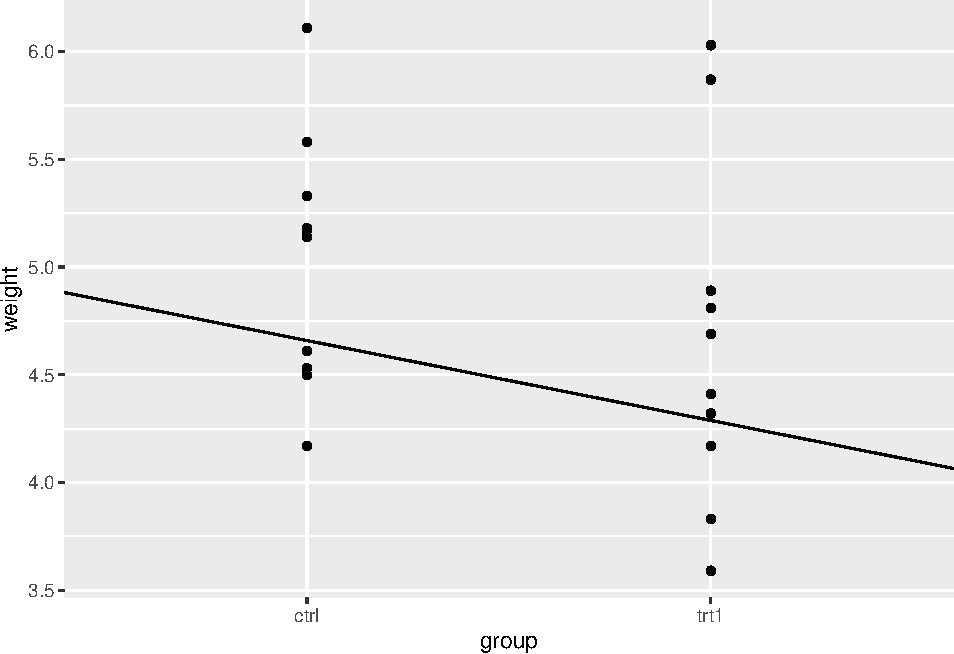
\includegraphics{intro_to_stats_files/figure-latex/unnamed-chunk-31-1.pdf}

Just looking at the plot makes the line look seem substantial than it is. Looking at the \(y\)-axis and the places where the line intercepts with the categories then we can see the difference is close to the coefficient.

\hypertarget{the-coefficient-and-the-mean-difference-between-groups-are-equivalent}{%
\subsection{The coefficient and the mean difference between groups are equivalent}\label{the-coefficient-and-the-mean-difference-between-groups-are-equivalent}}

Before we move along with our model, we should look at that coefficient of the group variable a bit more. As we're moving from the \texttt{ctrl} to \texttt{treatment} groups the coefficient tells us the size of the change. So does this mean that the coefficient is equivalent to other measures by which we can tell the difference in two groups - is it, for example equivalent to calculating the difference in the means of the groups? Short answer is yes! Let's look at that, recalling that the coefficient is \texttt{0.371}.

First get the means of the groups

\begin{Shaded}
\begin{Highlighting}[]
\NormalTok{mean_two_groups <-}\StringTok{ }\NormalTok{two_groups }\OperatorTok\StringTok{ }
\StringTok{  }\KeywordTok{group_by}\NormalTok{(group) }\OperatorTok\StringTok{ }
\StringTok{  }\KeywordTok{summarize}\NormalTok{(}\DataTypeTok{mean_wt =} \KeywordTok{mean}\NormalTok{(weight))}

\NormalTok{mean_two_groups}
\end{Highlighting}
\end{Shaded}

\begin{verbatim}
## # A tibble: 2 x 2
##   group mean_wt
##   <fct>   <dbl>
## 1 ctrl     5.03
## 2 trt1     4.66
\end{verbatim}

Now calculate the difference

\begin{Shaded}
\begin{Highlighting}[]
\FloatTok{5.03} \OperatorTok{-}\StringTok{ }\FloatTok{4.66}
\end{Highlighting}
\end{Shaded}

\begin{verbatim}
## [1] 0.37
\end{verbatim}

There you have it, the absolute values of each are very similar. You can use the coefficient as a way of finding the difference between the groups. Another handy feature of the linear model.

\hypertarget{the-p-value-of-the-co-efficient-tests-the-same-thing-as-a-t-test}{%
\subsection{\texorpdfstring{The \(p\)-value of the co-efficient tests the same thing as a \(t\)-test}{The p-value of the co-efficient tests the same thing as a t-test}}\label{the-p-value-of-the-co-efficient-tests-the-same-thing-as-a-t-test}}

We already know that the \(Pr(>|t|)\) value (\(p\)-value of the coefficient) tells us the probability that we would see the slope observed or greater in random samples if the real difference were 0. The two-sample \(t\)-test reports the probability that we would see the difference in means observed if the real difference were 0. So the two are very similar.

The \(p\)-value for the coefficient in the linear model was 0.249. How does this compare with a \(t\)-test?

\begin{Shaded}
\begin{Highlighting}[]
\KeywordTok{t.test}\NormalTok{(weight }\OperatorTok{~}\StringTok{ }\NormalTok{group, }\DataTypeTok{data =}\NormalTok{ two_groups)}
\end{Highlighting}
\end{Shaded}

\begin{verbatim}
## 
##  Welch Two Sample t-test
## 
## data:  weight by group
## t = 1.1913, df = 16.524, p-value = 0.2504
## alternative hypothesis: true difference in means is not equal to 0
## 95 percent confidence interval:
##  -0.2875162  1.0295162
## sample estimates:
## mean in group ctrl mean in group trt1 
##              5.032              4.661
\end{verbatim}

It is extremely close! In fact, as the sample size increase over about 15 it gets to be exact. So this is useful, we can use the linear model slope and \(p\)-value as a mental and practical alternative for thinking about the more complicated \(t\)-test.

All you have to understand is that you are looking at the slope of the line between the groups. If you don't see a slope of that size very often, then you can say its not likely that there's no difference \footnote{Again this is weak inference, but thats this type of statistics for you!}

\hypertarget{summary}{%
\section{Summary}\label{summary}}

Hopefully, this plot summarises how to look for differences between two groups using a linear model quite succinctly.

\begin{enumerate}
\def\labelenumi{\arabic{enumi}.}
\tightlist
\item
  Think of the line between the mean of the groups
\item
  Does the \(p\)-value tell you that you don't see a slope of this size often.
\end{enumerate}

So you just need the coefficient and the \(p\)-value from the linear model.
When we're thinking of the coefficient of the linear model for differences we're just asking something very similar to whether the line that joins the two means has a non-zero slope, given the error.

In a hypothesis test way, what we're asking amounts to the following two hypotheses:

\begin{itemize}
\tightlist
\item
  A flat line with slope of zero is equivalent to the Null hypothesis

  \begin{itemize}
  \tightlist
  \item
    \(H_{0}\) the group means are equal
  \end{itemize}
\item
  A \(p\)-value that suggests the slope is rare is equivalent to the Alternative hypothesis

  \begin{itemize}
  \tightlist
  \item
    \(H_{1}\) the group means are not equal
  \end{itemize}
\end{itemize}

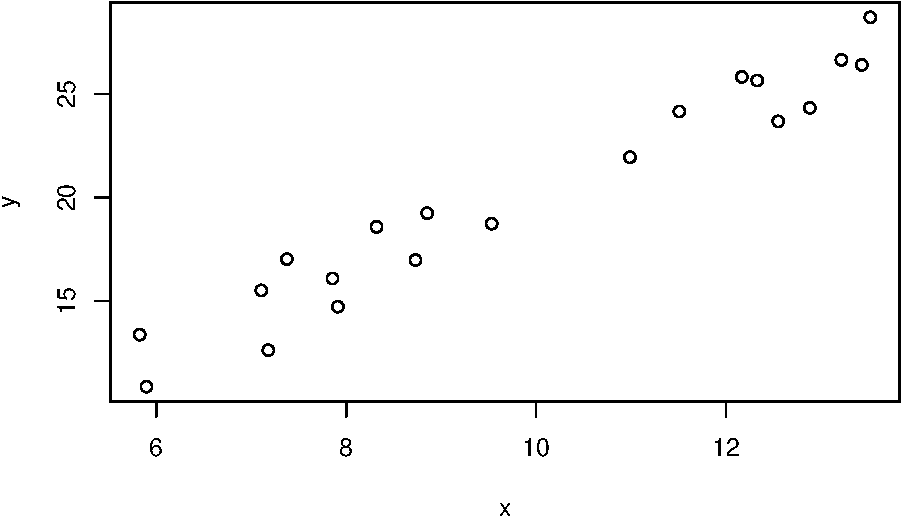
\includegraphics{intro_to_stats_files/figure-latex/unnamed-chunk-35-1.pdf}

\hypertarget{but-wasnt-the-t-test-just-easier}{%
\section{\texorpdfstring{But wasn't the \(t\)-test just easier?}{But wasn't the t-test just easier?}}\label{but-wasnt-the-t-test-just-easier}}

In the process we've been learning we used the \texttt{t.test()} function to calculate the \(p\)-value that tested the hypothesis that the true difference in the means was 0. This was pretty easy and we didn't have to think too hard, we just got the result. Why wouldn't we stick to just using that, if it's equivalent to the linear model? Because the linear model is a general answer to all these sorts of questions - one small set of techniques is useable in pretty much every situation, so in a wide range of experiments the statistics becomes a lot easier to understand, using it in place of all other tests uses basically the same set of skills we've applied here, there's not much more than we already know. Contrast this with the effort and time investment that it would take to learn the many different significance tests and all the different ways that they work.

The `learn all the significance tests' approach restricts us as scientists exploring our data in important ways. For example, the \(t\)-test (like all other tests) is a special case of the linear model, it can only be applied reliably when certain conditions are met. The \(t\)-test also `black-box's' the whole process, all the output you focus on is a \(p\)-value, in practice there isn't a whole lot to it and unless you study the innards of the \(t\)-test you can never compare two \(t\)-test results. Have you ever seen a \(p\)-value that you couldn't replicate or looked a bit suspect but couldn't work out why - using a linear model with all its measures of believability allows such comparisons to be done, you could say exactly why one model fit was better or worse than another and which hypotheses you can keep and reject more confidently. This is a very important point, by using linear models we also have a consistent way to criticise and evaluate our statistical conclusions - helping us to make better decisions and helping us to answer questions (perhaps from reviewers or group leaders) about the applicability and believeability.

Comparing more than two groups and looking at effects is basically the same thing, and we'll look at that in the next section.

\hypertarget{task}{%
\section{Task}\label{task}}

Make the PlantGrowth plot using \texttt{geom\_smooth()} with the error area.
geom\_smooth( aes(x = as.numeric(group), y = measurement), method = lm, colour = ``red'', linetype = ``dashed'')

\hypertarget{anova-and-linear-models}{%
\chapter{ANOVA and linear models}\label{anova-and-linear-models}}

\hypertarget{comparing-groups-in-a-single-variable}{%
\section{Comparing groups in a single variable}\label{comparing-groups-in-a-single-variable}}

In the last section we looked at using the linear model to compare two groups, in this section we'll look at using it to compare more than two. One thing to note is that we're still working with only one explanatory variable, the groups we are talking about are basically different values that the one variable can take. In the \texttt{PlantGrowth} data the variable is called \texttt{group} and the values it takes are \texttt{ctrl}, \texttt{trt1} and \texttt{trt2}.

TODO GLOSSARY EXPLANATORY VARIABLE, GROUPS LEVELS, FACTOR

You'll be pleased to know this is where the pay off comes. Any number of groups is no more complicated than the two we've already done.

We can visualise the process as simply being a case where we have more than one line to examine.

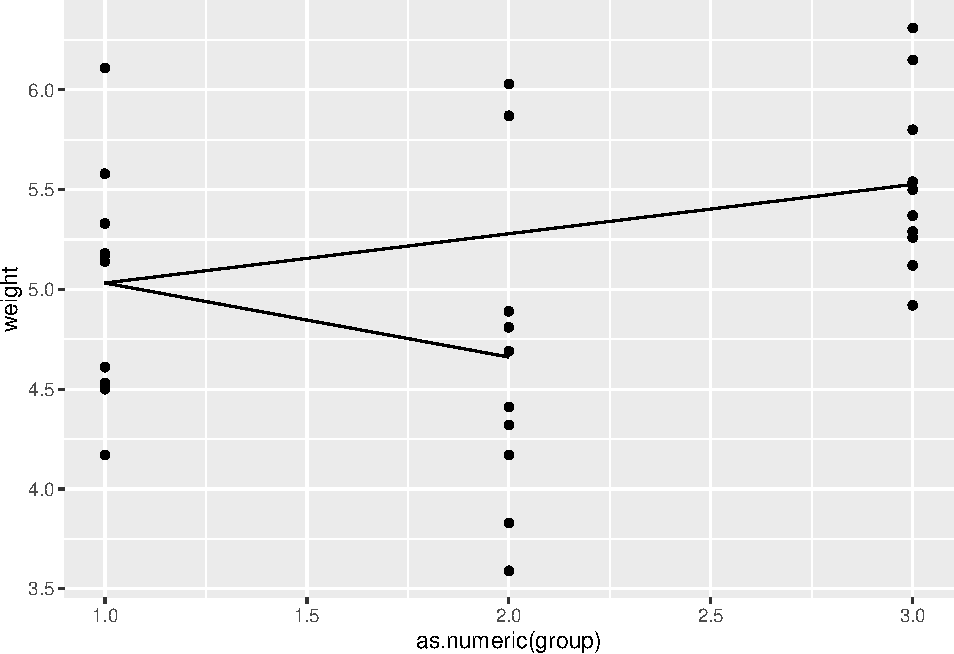
\includegraphics{intro_to_stats_files/figure-latex/unnamed-chunk-36-1.pdf}

In terms of a hypothesis test what we're asking amounts to the same as we saw with the \(t\)-test:

\begin{itemize}
\tightlist
\item
  All flat lines with slopes of zero is equivalent to the Null hypothesis

  \begin{itemize}
  \tightlist
  \item
    \(H_{0}\) the group means are \emph{all} equal
  \end{itemize}
\item
  At least one \(p\)-value that suggests the slope is rare is equivalent to the Alternative hypothesis

  \begin{itemize}
  \tightlist
  \item
    \(H_{1}\) the group means are not \emph{all} equal
  \end{itemize}
\end{itemize}

And putting that in a linear model is no different than before because we still have only one variable.

\begin{Shaded}
\begin{Highlighting}[]
\NormalTok{model <-}\StringTok{ }\KeywordTok{lm}\NormalTok{(weight }\OperatorTok{~}\StringTok{ }\NormalTok{group, }\DataTypeTok{data =}\NormalTok{ PlantGrowth)}
\KeywordTok{summary}\NormalTok{(model)}
\end{Highlighting}
\end{Shaded}

\begin{verbatim}
## 
## Call:
## lm(formula = weight ~ group, data = PlantGrowth)
## 
## Residuals:
##     Min      1Q  Median      3Q     Max 
## -1.0710 -0.4180 -0.0060  0.2627  1.3690 
## 
## Coefficients:
##             Estimate Std. Error t value Pr(>|t|)    
## (Intercept)   5.0320     0.1971  25.527   <2e-16 ***
## grouptrt1    -0.3710     0.2788  -1.331   0.1944    
## grouptrt2     0.4940     0.2788   1.772   0.0877 .  
## ---
## Signif. codes:  0 '***' 0.001 '**' 0.01 '*' 0.05 '.' 0.1 ' ' 1
## 
## Residual standard error: 0.6234 on 27 degrees of freedom
## Multiple R-squared:  0.2641, Adjusted R-squared:  0.2096 
## F-statistic: 4.846 on 2 and 27 DF,  p-value: 0.01591
\end{verbatim}

Great! so we handle the extra levels of the variable nearly perfectly. There are two lines of coefficient results, the first showing the gradient between the \texttt{ctrl} and \texttt{trt1} and the second showing the gradient between \texttt{ctrl} and \texttt{trt2}. The \texttt{ctrl} data has clearly been used as a common reference - this is the default design in the function, the first group in the data becomes the common reference. Here we get away with it, as we do want the first level to be the common reference. When you need to change the order, you can set the reference level explicitly.

\begin{Shaded}
\begin{Highlighting}[]
\NormalTok{df <-}\StringTok{ }\NormalTok{PlantGrowth}
\NormalTok{df}\OperatorTok{$}\NormalTok{group<-}\StringTok{ }\KeywordTok{relevel}\NormalTok{(df}\OperatorTok{$}\NormalTok{group, }\DataTypeTok{ref=}\StringTok{"trt2"}\NormalTok{)}
\NormalTok{model2 <-}\StringTok{ }\KeywordTok{lm}\NormalTok{(weight }\OperatorTok{~}\StringTok{ }\NormalTok{group  , }\DataTypeTok{data =}\NormalTok{ df,)}
\KeywordTok{summary}\NormalTok{(model2)}
\end{Highlighting}
\end{Shaded}

\begin{verbatim}
## 
## Call:
## lm(formula = weight ~ group, data = df)
## 
## Residuals:
##     Min      1Q  Median      3Q     Max 
## -1.0710 -0.4180 -0.0060  0.2627  1.3690 
## 
## Coefficients:
##             Estimate Std. Error t value Pr(>|t|)    
## (Intercept)   5.5260     0.1971  28.032  < 2e-16 ***
## groupctrl    -0.4940     0.2788  -1.772  0.08768 .  
## grouptrt1    -0.8650     0.2788  -3.103  0.00446 ** 
## ---
## Signif. codes:  0 '***' 0.001 '**' 0.01 '*' 0.05 '.' 0.1 ' ' 1
## 
## Residual standard error: 0.6234 on 27 degrees of freedom
## Multiple R-squared:  0.2641, Adjusted R-squared:  0.2096 
## F-statistic: 4.846 on 2 and 27 DF,  p-value: 0.01591
\end{verbatim}

And now we see the \texttt{trt2} as common reference against the \texttt{ctrl} and \texttt{trt1} groups.

In these data \texttt{ctrl\ vs\ trt1} appears to be significant according to the linear model \texttt{model1} and \texttt{trt1\ vs\ trt2} appears to be significant according to the linear model \texttt{model2} but we did need to create two models to do this. If this seems longwinded or illogical, then that's fair. The two models have the same data and specification so should have the same results in - it was really just the way we were ordering things in the data that was different. The real problem is just one of bookkeeping. The linear models are rich and not all the comparisons that can be done with them can easily be written in \texttt{summary(model)}. To answer specific questions from an analysis technique for getting specific comparisions (or contrasts in the statistics jargon) from linear models has been invented, that technique is called ANOVA (Analysis of Variance).

\hypertarget{one-way-comparisons}{%
\subsection{One-Way comparisons}\label{one-way-comparisons}}

The situation where we have just one variable is called a `One-Way' ANOVA.

Now that we have a solid way of thinking about contrasts as the slope between the categories, we can think of ANOVA as a tool for pulling out the significances in the best way. All we have to do is learn how to specify the contrasts for ANOVA.

Every time we do ANOVA we need a model to feed into it. Here's the most common way ANOVA is done in R, with the \texttt{aov()} and \texttt{TukeyHSD()} functions, you've probably seen this before.

\begin{Shaded}
\begin{Highlighting}[]
\NormalTok{ano <-}\StringTok{ }\KeywordTok{aov}\NormalTok{(model)}
\KeywordTok{TukeyHSD}\NormalTok{(ano)}
\end{Highlighting}
\end{Shaded}

\begin{verbatim}
##   Tukey multiple comparisons of means
##     95% family-wise confidence level
## 
## Fit: aov(formula = model)
## 
## $group
##             diff        lwr       upr     p adj
## trt1-ctrl -0.371 -1.0622161 0.3202161 0.3908711
## trt2-ctrl  0.494 -0.1972161 1.1852161 0.1979960
## trt2-trt1  0.865  0.1737839 1.5562161 0.0120064
\end{verbatim}

It seems to do the job, though the `flavour' of ANOVA it does is limited and applies only when the standard assumptions of ANOVA are met.

A better alternative is the \texttt{multcomp} package function \texttt{glht()} (general linear model hypothesis test), which is more flexible with respect to which designs and contrasts you can get out, at the expense of being a little more complicated. The basic case is straightforward though.

\begin{Shaded}
\begin{Highlighting}[]
\KeywordTok{library}\NormalTok{(multcomp)}
\NormalTok{tested <-}\StringTok{ }\KeywordTok{glht}\NormalTok{(model, }\DataTypeTok{linfct =} \KeywordTok{mcp}\NormalTok{(}\DataTypeTok{group =} \StringTok{"Tukey"}\NormalTok{))}
\KeywordTok{summary}\NormalTok{(tested)}
\end{Highlighting}
\end{Shaded}

\begin{verbatim}
## 
##   Simultaneous Tests for General Linear Hypotheses
## 
## Multiple Comparisons of Means: Tukey Contrasts
## 
## 
## Fit: lm(formula = weight ~ group, data = PlantGrowth)
## 
## Linear Hypotheses:
##                  Estimate Std. Error t value Pr(>|t|)  
## trt1 - ctrl == 0  -0.3710     0.2788  -1.331    0.391  
## trt2 - ctrl == 0   0.4940     0.2788   1.772    0.198  
## trt2 - trt1 == 0   0.8650     0.2788   3.103    0.012 *
## ---
## Signif. codes:  0 '***' 0.001 '**' 0.01 '*' 0.05 '.' 0.1 ' ' 1
## (Adjusted p values reported -- single-step method)
\end{verbatim}

The \texttt{linfct} option just takes a specification of the things to be tested, and the \texttt{mcp()} function is a helper that generates the comparison based on a text description, here that the variable \texttt{group} should be analysed by `Tukey'.

By printing the summary we see the contrast hypotheses writ explicitly (e.g.~the difference between \texttt{ctrl} and \texttt{trt1} is 0) and the conclusions: there is no evidence to suggest either treatment is different from the control, but the difference we observe between the \texttt{group1} and \texttt{group2} occurs by chance only about 1.2 percent of the time.

We'll see more of how to use \texttt{glht()} as we go.

\hypertarget{comparing-groups-in-multiple-variables}{%
\section{Comparing groups in multiple variables}\label{comparing-groups-in-multiple-variables}}

Often we'll have experimental data where we have more than one explanatory variable, for example, \texttt{temperature} and \texttt{fertiliser} and want to know the effects of each on a response variable like \texttt{yield}.

\hypertarget{two-way-comparisons}{%
\subsection{Two-Way comparisons}\label{two-way-comparisons}}

Such a situation is complicated over the single case as we have more the possibility of an interaction between the variables to consider. The case where we want to look at ANOVA for models with an two variables and an interaction effect is called a \texttt{Two-Way\ ANOVA}.

Let's work through an example that highlights that. Here's some data on reported enjoyment of some food, with different condiments added

\begin{tabular}{l|l|r}
\hline
Food & Condiment & Enjoyment\\
\hline
Hot Dog & Mustard & 94.30379\\
\hline
Hot Dog & Mustard & 87.33326\\
\hline
Ice Cream & Mustard & 66.45707\\
\hline
Ice Cream & Chocolate Sauce & 95.22787\\
\hline
Ice Cream & Mustard & 56.58818\\
\hline
\end{tabular}

Looking at those in the way we have already - each variable individually - then we would generate the following plots and lines to examine.

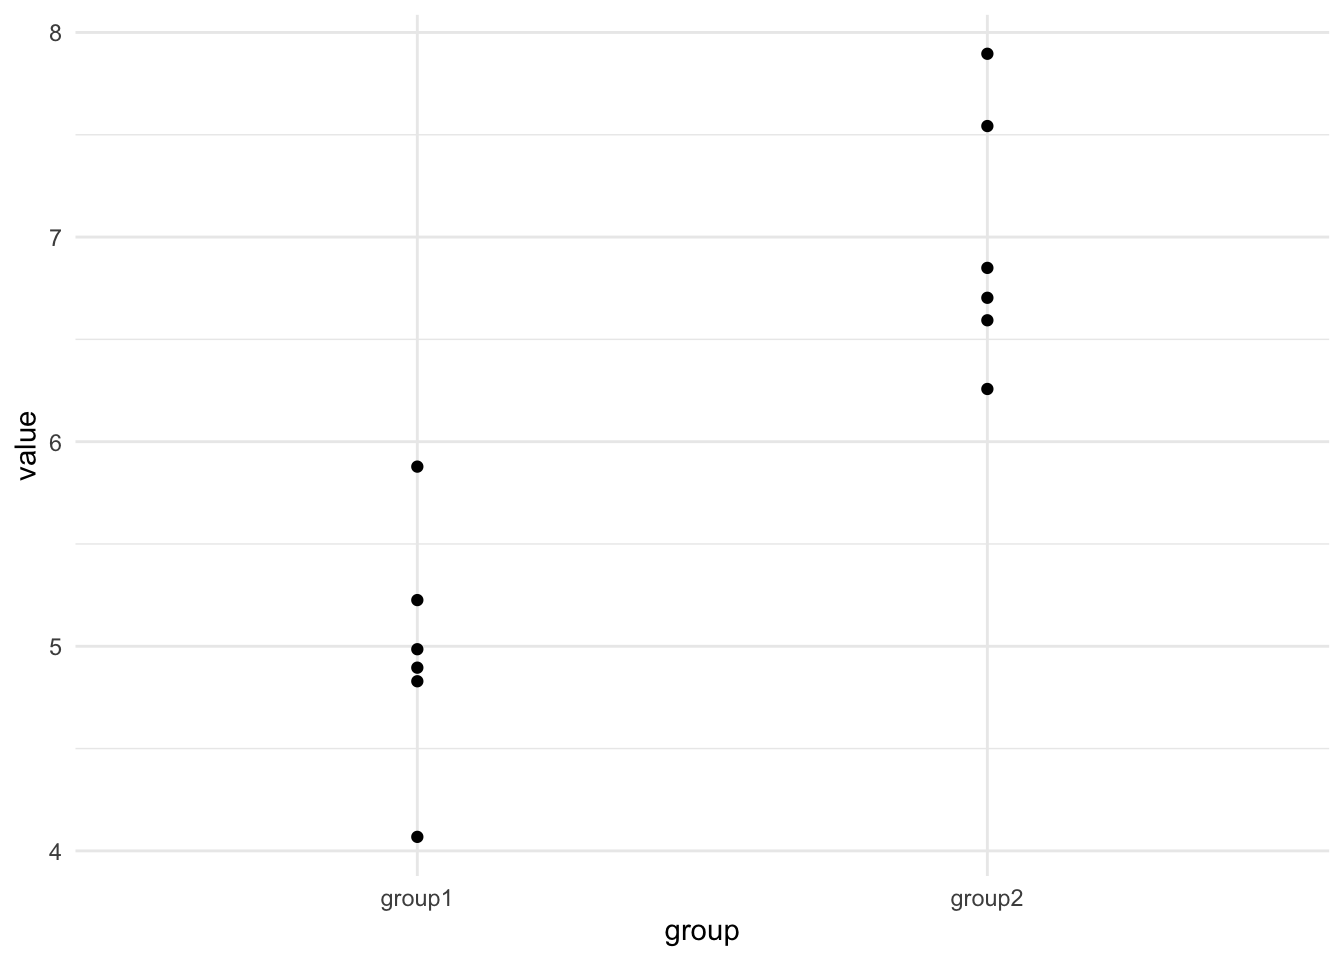
\includegraphics[width=0.5\linewidth]{intro_to_stats_files/figure-latex/unnamed-chunk-42-1} 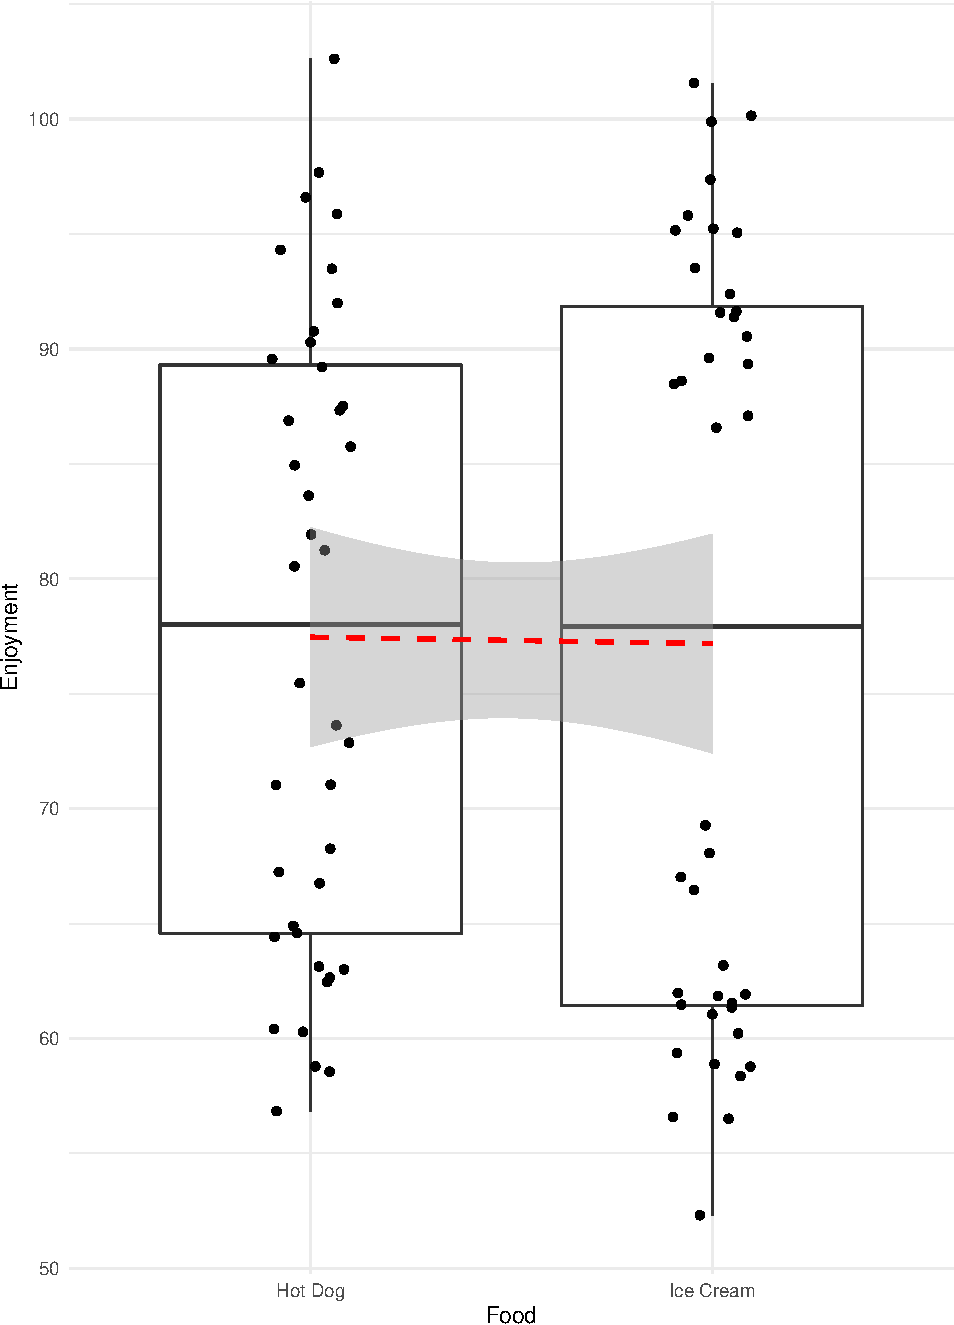
\includegraphics[width=0.5\linewidth]{intro_to_stats_files/figure-latex/unnamed-chunk-42-2}

Without rushing ahead to do the modelling, we see that chocolate sauce has a slightly greater effect on enjoyment than mustard, whereas the enjoyment of the two food types is the same. So the conclusion would be `use chocolate sauce to enhance your enjoyment of Hot Dogs or Ice Cream'.

Let's see what the model says, in specifying the second variable can be added with a \texttt{+} and

\begin{Shaded}
\begin{Highlighting}[]
\NormalTok{model_}\DecValTok{1}\NormalTok{ <-}\StringTok{ }\KeywordTok{lm}\NormalTok{(Enjoyment }\OperatorTok{~}\StringTok{ }\NormalTok{Food }\OperatorTok{+}\StringTok{ }\NormalTok{Condiment, }\DataTypeTok{data =}\NormalTok{ food)}
\KeywordTok{summary}\NormalTok{(model_}\DecValTok{1}\NormalTok{)}
\end{Highlighting}
\end{Shaded}

\begin{verbatim}
## 
## Call:
## lm(formula = Enjoyment ~ Food + Condiment, data = food)
## 
## Residuals:
##      Min       1Q   Median       3Q      Max 
## -23.0067 -14.3016   0.5382  13.4187  27.0218 
## 
## Coefficients:
##                  Estimate Std. Error t value Pr(>|t|)    
## (Intercept)       79.3237     2.9278  27.093   <2e-16 ***
## FoodIce Cream     -0.2826     3.3807  -0.084    0.934    
## CondimentMustard  -3.7251     3.3807  -1.102    0.274    
## ---
## Signif. codes:  0 '***' 0.001 '**' 0.01 '*' 0.05 '.' 0.1 ' ' 1
## 
## Residual standard error: 15.12 on 77 degrees of freedom
## Multiple R-squared:  0.01561,    Adjusted R-squared:  -0.009958 
## F-statistic: 0.6105 on 2 and 77 DF,  p-value: 0.5457
\end{verbatim}

The summary isn't promising, it looks like neither is significant. Let's do the ANOVA and get conclusive proof.

The call to \texttt{glht()} is a bit more complicated, but not much

\begin{Shaded}
\begin{Highlighting}[]
\KeywordTok{summary}\NormalTok{(}\KeywordTok{glht}\NormalTok{(model_}\DecValTok{1}\NormalTok{, }\DataTypeTok{linfct =} \KeywordTok{mcp}\NormalTok{(}\DataTypeTok{Food =} \StringTok{"Tukey"}\NormalTok{, }\DataTypeTok{Condiment =} \StringTok{"Tukey"}\NormalTok{) ) )}
\end{Highlighting}
\end{Shaded}

\begin{verbatim}
## 
##   Simultaneous Tests for General Linear Hypotheses
## 
## Multiple Comparisons of Means: Tukey Contrasts
## 
## 
## Fit: lm(formula = Enjoyment ~ Food + Condiment, data = food)
## 
## Linear Hypotheses:
##                                           Estimate Std. Error t value Pr(>|t|)
## Food: Ice Cream - Hot Dog == 0             -0.2826     3.3807  -0.084    0.996
## Condiment: Mustard - Chocolate Sauce == 0  -3.7251     3.3807  -1.102    0.471
## (Adjusted p values reported -- single-step method)
\end{verbatim}

Neither factor seems to be significant. Hmm. This seems like a slightly strange conclusion - and it is. The presence of two variables is confusing this approach. Look at what we get if we split the data by the two variables at once.

\hypertarget{interaction-between-variables}{%
\subsection{Interaction between variables}\label{interaction-between-variables}}

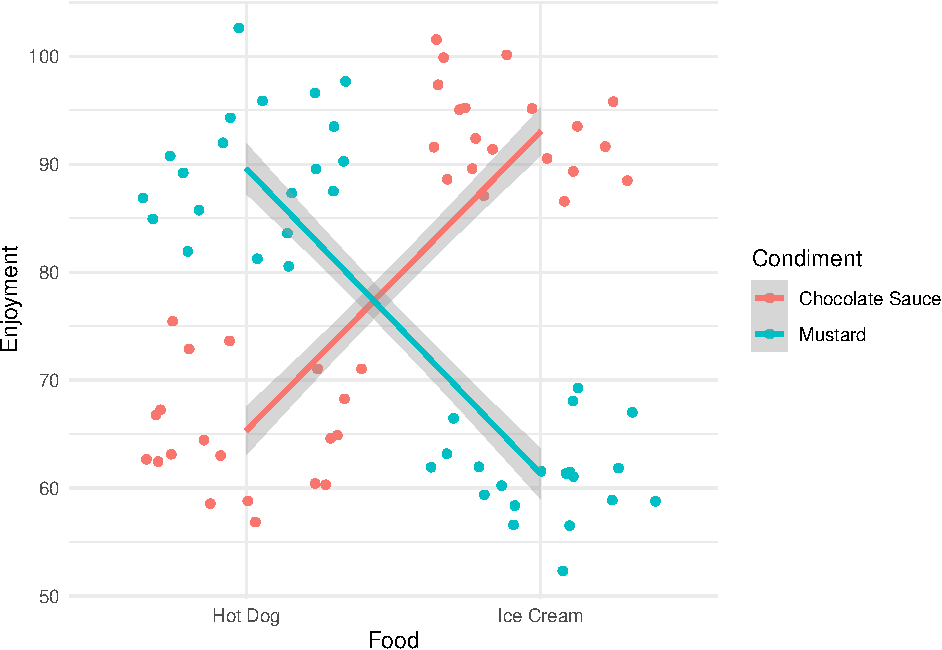
\includegraphics{intro_to_stats_files/figure-latex/unnamed-chunk-45-1.pdf} 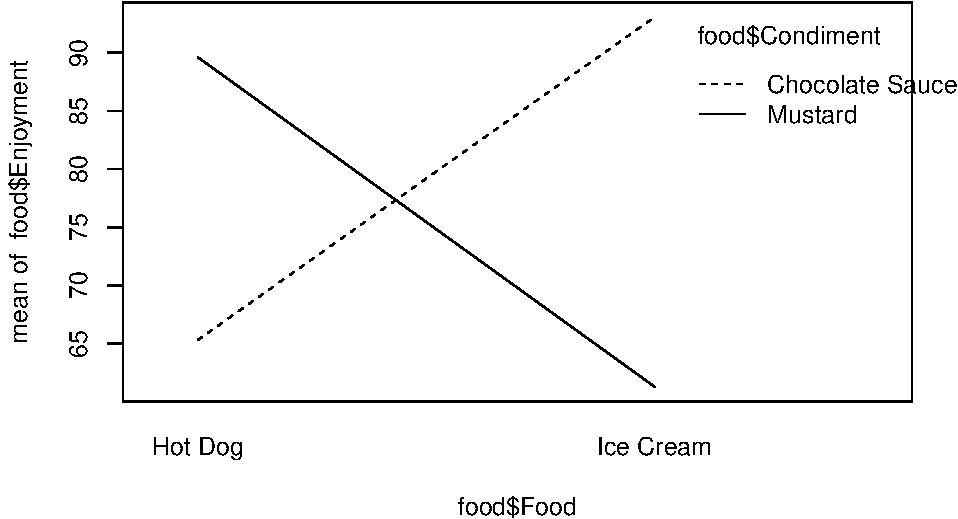
\includegraphics{intro_to_stats_files/figure-latex/unnamed-chunk-45-2.pdf}

Ok! That's very different and very much clearer. The enjoyment is very much dependent on the combination of food and condiment. This is a classic case of interaction between variables. You get results that are conditional on the combined values of the variables.

The cross-over of the lines is a visual diagnostic of the presence of an interaction effect.

\hypertarget{modelling-an-interaction-effect}{%
\subsection{Modelling an interaction effect}\label{modelling-an-interaction-effect}}

The interaction effect should be checked for in the linear model. It is quite easy to check for and requires a slight extension to syntax. An interaction can be specified with the \texttt{:}.

\begin{Shaded}
\begin{Highlighting}[]
\NormalTok{interaction_model <-}\StringTok{ }\KeywordTok{lm}\NormalTok{(Enjoyment }\OperatorTok{~}\StringTok{ }\NormalTok{Food }\OperatorTok{+}\StringTok{ }\NormalTok{Condiment }\OperatorTok{+}\StringTok{ }\NormalTok{Food}\OperatorTok{:}\NormalTok{Condiment, }\DataTypeTok{data =}\NormalTok{ food)}
\end{Highlighting}
\end{Shaded}

(there is also a short hand that allows the whole thing to be specified in one term \texttt{*}, which is used like \texttt{lm(Enjoyment\ \textasciitilde{}\ Food\ *\ Condiment,\ data=food)})

and when we print the \texttt{summary()} we get the book-keeping issue, but we can see the usual stuff.

\begin{Shaded}
\begin{Highlighting}[]
\KeywordTok{summary}\NormalTok{(interaction_model)}
\end{Highlighting}
\end{Shaded}

\begin{verbatim}
## 
## Call:
## lm(formula = Enjoyment ~ Food + Condiment + Food:Condiment, data = food)
## 
## Residuals:
##    Min     1Q Median     3Q    Max 
## -9.068 -3.068 -0.407  2.802 13.015 
## 
## Coefficients:
##                                Estimate Std. Error t value Pr(>|t|)    
## (Intercept)                      65.317      1.120   58.34   <2e-16 ***
## FoodIce Cream                    27.731      1.583   17.52   <2e-16 ***
## CondimentMustard                 24.289      1.583   15.34   <2e-16 ***
## FoodIce Cream:CondimentMustard  -56.028      2.239  -25.02   <2e-16 ***
## ---
## Signif. codes:  0 '***' 0.001 '**' 0.01 '*' 0.05 '.' 0.1 ' ' 1
## 
## Residual standard error: 5.007 on 76 degrees of freedom
## Multiple R-squared:  0.8935, Adjusted R-squared:  0.8892 
## F-statistic: 212.4 on 3 and 76 DF,  p-value: < 2.2e-16
\end{verbatim}

This seems much more like what we expect from the graph, significance everywhere! Basically what the summary is saying is that the Food, Condiment and both together have an effect on the reported enjoyment. But are the contrasts presented here really all the ones we're interested in? They aren't here, and this is generally the case so we need to know how to extract them. First we must decide what the contrasts we're going to check must be. In our linear model way of thinking this means which lines do we want to test for zero slopes? There can be many lines we could imagine depending on how we decide to group the data and the number of variables that we have. Let's define which we'll look at before we begin.

Let's see whether food alone or condiment alone has an effect. This would be like the first situation we looked at,

\begin{Shaded}
\begin{Highlighting}[]
\NormalTok{plot_condiment}
\end{Highlighting}
\end{Shaded}

\begin{verbatim}
## `geom_smooth()` using formula 'y ~ x'
\end{verbatim}

\begin{Shaded}
\begin{Highlighting}[]
\NormalTok{plot_food}
\end{Highlighting}
\end{Shaded}

\begin{verbatim}
## `geom_smooth()` using formula 'y ~ x'
\end{verbatim}

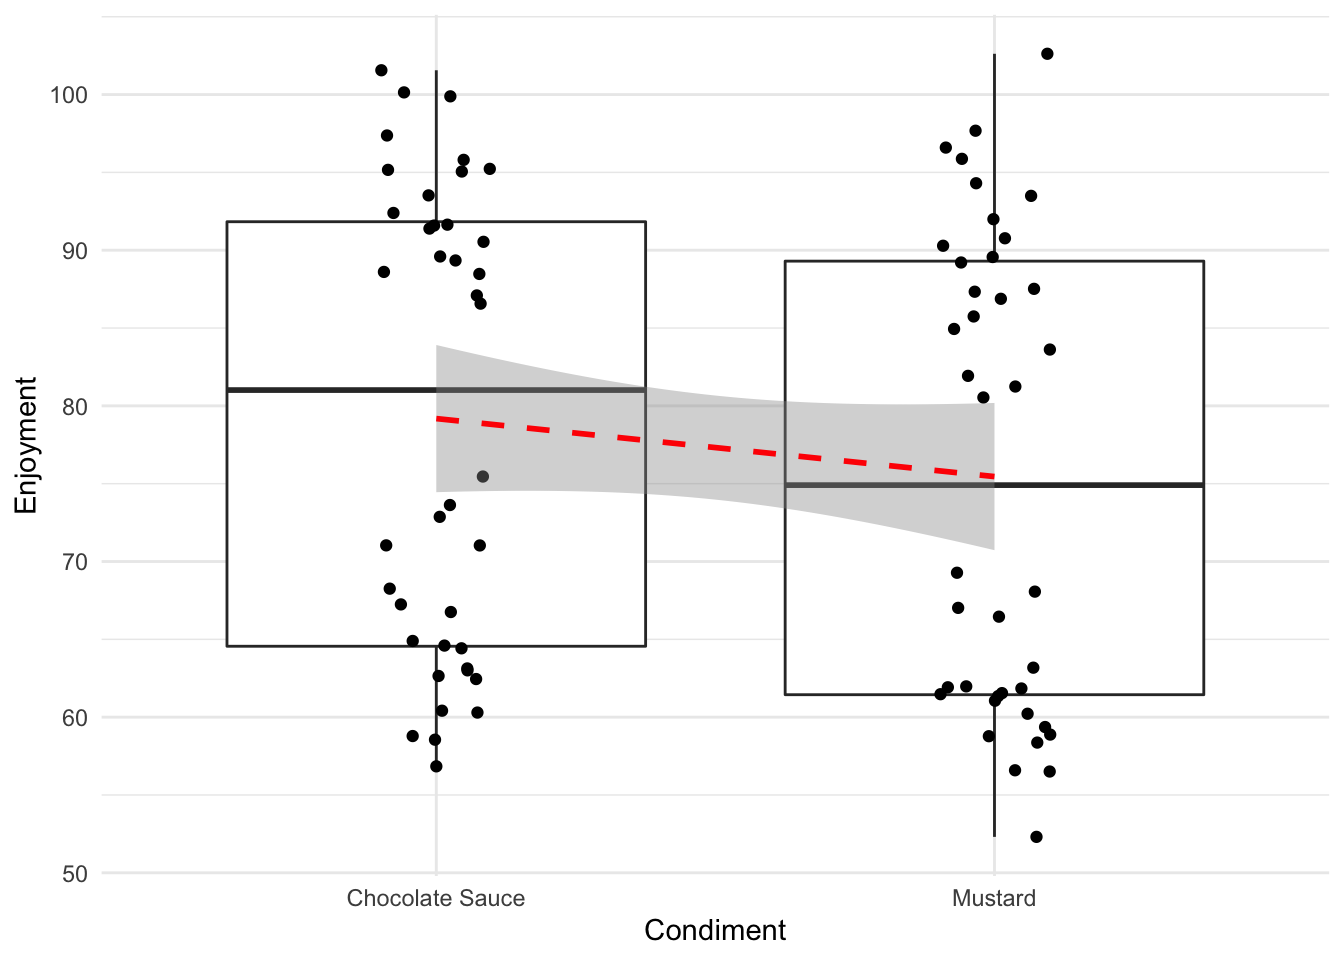
\includegraphics[width=0.5\linewidth]{intro_to_stats_files/figure-latex/unnamed-chunk-48-1} 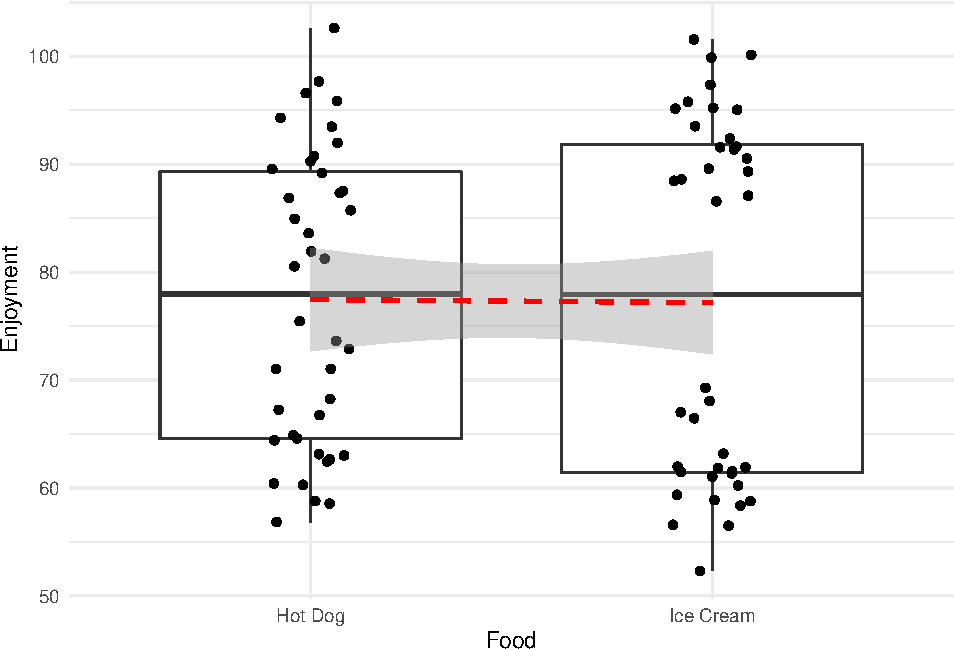
\includegraphics[width=0.5\linewidth]{intro_to_stats_files/figure-latex/unnamed-chunk-48-2}

in the way that the output we've seen so far has it, this would be

Hot Dog - Ice Cream == 0
Chocolate Sauce - Mustard == 0

Let's also see whether \texttt{food\ *\ condiment} has an effect. This would be like the interaction situation.

Hot Dog:Mustard - Ice Cream:Mustard == 0
Hot Dog:Chocolate Sauce - Ice Cream:Chocolate Sauce == 0

\begin{Shaded}
\begin{Highlighting}[]
\NormalTok{plot_interaction}
\end{Highlighting}
\end{Shaded}

\begin{verbatim}
## `geom_smooth()` using formula 'y ~ x'
\end{verbatim}

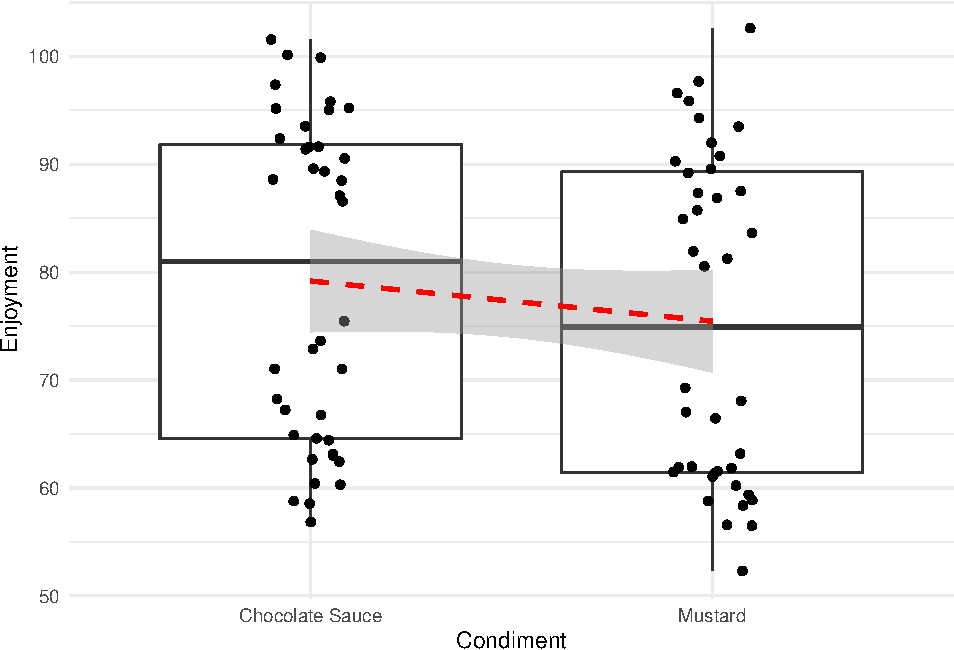
\includegraphics{intro_to_stats_files/figure-latex/unnamed-chunk-49-1.pdf}

So we have four lines of interest to look at - four contrasts. For the two main non-interaction effects we can look at these as we've done before, using the \texttt{mcp()} function.

\begin{Shaded}
\begin{Highlighting}[]
\KeywordTok{summary}\NormalTok{(}
  \KeywordTok{glht}\NormalTok{(interaction_model, }\DataTypeTok{linfct =} \KeywordTok{mcp}\NormalTok{(}
    \DataTypeTok{Food =} \StringTok{"Tukey"}\NormalTok{,}
    \DataTypeTok{Condiment =} \StringTok{"Tukey"}
\NormalTok{  ))}
\NormalTok{)}
\end{Highlighting}
\end{Shaded}

\begin{verbatim}
## Warning in mcp2matrix(model, linfct = linfct): covariate interactions found --
## default contrast might be inappropriate

## Warning in mcp2matrix(model, linfct = linfct): covariate interactions found --
## default contrast might be inappropriate
\end{verbatim}

\begin{verbatim}
## 
##   Simultaneous Tests for General Linear Hypotheses
## 
## Multiple Comparisons of Means: Tukey Contrasts
## 
## 
## Fit: lm(formula = Enjoyment ~ Food + Condiment + Food:Condiment, data = food)
## 
## Linear Hypotheses:
##                                           Estimate Std. Error t value Pr(>|t|)
## Food: Ice Cream - Hot Dog == 0              27.731      1.583   17.52   <1e-10
## Condiment: Mustard - Chocolate Sauce == 0   24.289      1.583   15.34   <1e-10
##                                              
## Food: Ice Cream - Hot Dog == 0            ***
## Condiment: Mustard - Chocolate Sauce == 0 ***
## ---
## Signif. codes:  0 '***' 0.001 '**' 0.01 '*' 0.05 '.' 0.1 ' ' 1
## (Adjusted p values reported -- single-step method)
\end{verbatim}

\hypertarget{doing-all-pairwise-interactions}{%
\subsubsection{Doing all pairwise interactions}\label{doing-all-pairwise-interactions}}

Although we're interested in only two specific interactions, usually it's easier to do all pairwise comparisons in one step, as we don't often have so many interacting variables that it gets unwieldy. To do this we must add an interaction column to our data and model that.

\begin{Shaded}
\begin{Highlighting}[]
\NormalTok{food_}\DecValTok{2}\NormalTok{ <-}\StringTok{ }\NormalTok{food }\OperatorTok\StringTok{ }\KeywordTok{mutate}\NormalTok{(}\DataTypeTok{FoodCondiment =} \KeywordTok{interaction}\NormalTok{(Food, Condiment))}

\NormalTok{int_model2 <-}\StringTok{ }\KeywordTok{lm}\NormalTok{(Enjoyment }\OperatorTok{~}\StringTok{ }\NormalTok{FoodCondiment, }\DataTypeTok{data =}\NormalTok{ food_}\DecValTok{2}\NormalTok{)}

\KeywordTok{summary}\NormalTok{(}\KeywordTok{glht}\NormalTok{(int_model2, }\DataTypeTok{linfct =} \KeywordTok{mcp}\NormalTok{(}\DataTypeTok{FoodCondiment =} \StringTok{"Tukey"}\NormalTok{)))}
\end{Highlighting}
\end{Shaded}

\begin{verbatim}
## 
##   Simultaneous Tests for General Linear Hypotheses
## 
## Multiple Comparisons of Means: Tukey Contrasts
## 
## 
## Fit: lm(formula = Enjoyment ~ FoodCondiment, data = food_2)
## 
## Linear Hypotheses:
##                                                          Estimate Std. Error
## Ice Cream.Chocolate Sauce - Hot Dog.Chocolate Sauce == 0   27.731      1.583
## Hot Dog.Mustard - Hot Dog.Chocolate Sauce == 0             24.289      1.583
## Ice Cream.Mustard - Hot Dog.Chocolate Sauce == 0           -4.008      1.583
## Hot Dog.Mustard - Ice Cream.Chocolate Sauce == 0           -3.442      1.583
## Ice Cream.Mustard - Ice Cream.Chocolate Sauce == 0        -31.739      1.583
## Ice Cream.Mustard - Hot Dog.Mustard == 0                  -28.297      1.583
##                                                          t value Pr(>|t|)    
## Ice Cream.Chocolate Sauce - Hot Dog.Chocolate Sauce == 0  17.515   <0.001 ***
## Hot Dog.Mustard - Hot Dog.Chocolate Sauce == 0            15.341   <0.001 ***
## Ice Cream.Mustard - Hot Dog.Chocolate Sauce == 0          -2.531   0.0635 .  
## Hot Dog.Mustard - Ice Cream.Chocolate Sauce == 0          -2.174   0.1397    
## Ice Cream.Mustard - Ice Cream.Chocolate Sauce == 0       -20.047   <0.001 ***
## Ice Cream.Mustard - Hot Dog.Mustard == 0                 -17.872   <0.001 ***
## ---
## Signif. codes:  0 '***' 0.001 '**' 0.01 '*' 0.05 '.' 0.1 ' ' 1
## (Adjusted p values reported -- single-step method)
\end{verbatim}

And now we can see all possible interaction groupings and lines. We can see that the signficances make good sense. The Hot Dog and Mustard is no more enjoyable than the Ice Cream and Chocolate Sauce, the Ice Cream and Mustard is no more enjoyable than the Hot Dog and Chocolate Sauce and all the other match and mismatch food and condiments are as we might expect from this very obviously loaded example.

We said we wanted to look specifically at the interaction between the Hot Dog with Mustard and Ice Cream with Mustard - we can see that there is a significant difference in enjoyment, about 17 points. Similarly Hot Dog with Chocolate Sauce is less enjoyable than Ice Cream with Chocolate Sauce, by about 27 points.

\hypertarget{testing-specific-interactions}{%
\subsubsection{Testing specific interactions}\label{testing-specific-interactions}}

The table above, as ever, is a bit rich and confusing, you can get a simpler output at the expense of some more work. For the two sets of interactions we're interested in we can look at them specifically but naming them explicitly in \texttt{glht} is trickier than we've done so far.

We have to specify a matrix of comparisons ourselves. The first step is to work out all the different interactions of the levels of the \texttt{food*condiment} interaction term. We can do that with the \texttt{interaction()} function

\begin{Shaded}
\begin{Highlighting}[]
\NormalTok{f_c_interactions <-}\StringTok{ }\KeywordTok{interaction}\NormalTok{(food}\OperatorTok{$}\NormalTok{Food, food}\OperatorTok{$}\NormalTok{Condiment, }\DataTypeTok{sep=}\StringTok{":"}\NormalTok{)}
\KeywordTok{head}\NormalTok{(f_c_interactions)}
\end{Highlighting}
\end{Shaded}

\begin{verbatim}
## [1] Hot Dog:Mustard Hot Dog:Mustard Hot Dog:Mustard Hot Dog:Mustard
## [5] Hot Dog:Mustard Hot Dog:Mustard
## 4 Levels: Hot Dog:Chocolate Sauce ... Ice Cream:Mustard
\end{verbatim}

We can see that this is just a factor object with all the combinations of \texttt{Food} and \texttt{Condiment}. Using the \texttt{levels()} function gives us all the unique values in the order that R will use them.

\begin{Shaded}
\begin{Highlighting}[]
\KeywordTok{levels}\NormalTok{(f_c_interactions)}
\end{Highlighting}
\end{Shaded}

\begin{verbatim}
## [1] "Hot Dog:Chocolate Sauce"   "Ice Cream:Chocolate Sauce"
## [3] "Hot Dog:Mustard"           "Ice Cream:Mustard"
\end{verbatim}

Now we can make the matrix, our eventual matrix will look like this

\begin{tabular}{l|r|r|r|r}
\hline
  & Hot Dog:Chocolate Sauce & Ice Cream:Chocolate Sauce & Hot Dog:Mustard & Ice Cream:Mustard\\
\hline
Hot Dog:Mustard - Ice Cream:Mustard & 0 & 0 & 1 & -1\\
\hline
Hot Dog:Chocolate Sauce - Ice Cream:Chocolate Sauce & 1 & -1 & 0 & 0\\
\hline
\end{tabular}

We can see that there is a row per comparison and a column per possible interaction. At the intersection we write a zero if we don't want to include that possible interaction in the contrast, a 1 if we want it to be the first part and a -1 if we want it to be the second part (IE, the part after the minus sign).

As the \texttt{levels()} function gives us the order, we set up the rows one by one and join them together.

\begin{Shaded}
\begin{Highlighting}[]
\NormalTok{HD.M_IC.M <-}\StringTok{ }\KeywordTok{c}\NormalTok{(}\DecValTok{0}\NormalTok{,}\DecValTok{0}\NormalTok{,}\DecValTok{1}\NormalTok{,}\OperatorTok{-}\DecValTok{1}\NormalTok{)}
\NormalTok{HD.C_IC.C <-}\StringTok{ }\KeywordTok{c}\NormalTok{(}\DecValTok{1}\NormalTok{,}\OperatorTok{-}\DecValTok{1}\NormalTok{,}\DecValTok{0}\NormalTok{,}\DecValTok{0}\NormalTok{)}
\end{Highlighting}
\end{Shaded}

Now we can stick them together, use the \texttt{levels()} function as the column names and add row names. Note you can call the rows what you like, so you dont have to use the long names, but the columns \emph{must} be named and ordered according to the \texttt{levels()} function

\begin{Shaded}
\begin{Highlighting}[]
\NormalTok{contr_of_interest <-}\StringTok{ }\KeywordTok{rbind}\NormalTok{(HD.M_IC.M, HD.C_IC.C)}
\KeywordTok{colnames}\NormalTok{(contr_of_interest) <-}\StringTok{ }\KeywordTok{levels}\NormalTok{(f_c_interactions)}
\KeywordTok{rownames}\NormalTok{(contr_of_interest) <-}\StringTok{ }\KeywordTok{c}\NormalTok{(}\StringTok{"HD:M - IC:M"}\NormalTok{,}
          \StringTok{"HD:CS - IC:CS"}\NormalTok{)}

\NormalTok{contr_of_interest}
\end{Highlighting}
\end{Shaded}

\begin{verbatim}
##               Hot Dog:Chocolate Sauce Ice Cream:Chocolate Sauce Hot Dog:Mustard
## HD:M - IC:M                         0                         0               1
## HD:CS - IC:CS                       1                        -1               0
##               Ice Cream:Mustard
## HD:M - IC:M                  -1
## HD:CS - IC:CS                 0
\end{verbatim}

Now we can do the test using the custom matrix.

\begin{Shaded}
\begin{Highlighting}[]
\KeywordTok{summary}\NormalTok{(}\KeywordTok{glht}\NormalTok{( interaction_model, }\DataTypeTok{linfct =}\NormalTok{ contr_of_interest))}
\end{Highlighting}
\end{Shaded}

\begin{verbatim}
## 
##   Simultaneous Tests for General Linear Hypotheses
## 
## Fit: lm(formula = Enjoyment ~ Food + Condiment + Food:Condiment, data = food)
## 
## Linear Hypotheses:
##                    Estimate Std. Error t value Pr(>|t|)    
## HD:M - IC:M == 0     80.317      3.540   22.69   <1e-10 ***
## HD:CS - IC:CS == 0   37.585      2.503   15.01   <1e-10 ***
## ---
## Signif. codes:  0 '***' 0.001 '**' 0.01 '*' 0.05 '.' 0.1 ' ' 1
## (Adjusted p values reported -- single-step method)
\end{verbatim}

And there we have the specific interaction contrasts.

H0: The means of all month groups are equal
H1: The mean of at least one month group is different

H0: The means of the gender groups are equal
H1: The means of the gender groups are different

H0: There is no interaction between the month and gender
H1: There is interaction between the month and gender

\hypertarget{occams-razor}{%
\section{Occam's Razor}\label{occams-razor}}

Simplest model - Compost data
Add compost data to package.
--------------------------------------

tasks one way, two way and three way anova on palmers penguins
use \texttt{interaction.plot()} on food to reproduce interaction plot. What would no interaction look like (flat lines)
compare and keep simplest model.

Look at some results tables to see how much effects are (examine the estimate columns).

\begin{Shaded}
\begin{Highlighting}[]
\KeywordTok{library}\NormalTok{(palmerpenguins)}
\KeywordTok{summary}\NormalTok{(penguins)}
\end{Highlighting}
\end{Shaded}

\begin{verbatim}
##       species          island    bill_length_mm  bill_depth_mm  
##  Adelie   :152   Biscoe   :168   Min.   :32.10   Min.   :13.10  
##  Chinstrap: 68   Dream    :124   1st Qu.:39.23   1st Qu.:15.60  
##  Gentoo   :124   Torgersen: 52   Median :44.45   Median :17.30  
##                                  Mean   :43.92   Mean   :17.15  
##                                  3rd Qu.:48.50   3rd Qu.:18.70  
##                                  Max.   :59.60   Max.   :21.50  
##                                  NA's   :2       NA's   :2      
##  flipper_length_mm  body_mass_g       sex     
##  Min.   :172.0     Min.   :2700   female:165  
##  1st Qu.:190.0     1st Qu.:3550   male  :168  
##  Median :197.0     Median :4050   NA's  : 11  
##  Mean   :200.9     Mean   :4202               
##  3rd Qu.:213.0     3rd Qu.:4750               
##  Max.   :231.0     Max.   :6300               
##  NA's   :2         NA's   :2
\end{verbatim}

\begin{Shaded}
\begin{Highlighting}[]
\KeywordTok{ggplot}\NormalTok{(penguins) }\OperatorTok{+}\StringTok{ }\KeywordTok{aes}\NormalTok{(species, bill_length_mm) }\OperatorTok{+}\StringTok{ }\KeywordTok{geom_jitter}\NormalTok{(}\KeywordTok{aes}\NormalTok{(}\DataTypeTok{colour =}\NormalTok{ sex), }\DataTypeTok{position =} \KeywordTok{position_dodge}\NormalTok{(}\DataTypeTok{width =} \FloatTok{0.5}\NormalTok{))}
\NormalTok{model <-}\StringTok{ }\KeywordTok{lm}\NormalTok{(bill_length_mm }\OperatorTok{~}\StringTok{ }\NormalTok{species }\OperatorTok{+}\StringTok{ }\NormalTok{sex, }\DataTypeTok{data =}\NormalTok{ penguins)}
\KeywordTok{summary}\NormalTok{(model)}
\CommentTok{# setup comparisons explicitly}
\NormalTok{comps <-}\StringTok{ }\KeywordTok{mcp}\NormalTok{( }\DataTypeTok{species =} \KeywordTok{c}\NormalTok{(}\StringTok{"Chinstrap - Gentoo = 0"}\NormalTok{,}
                          \StringTok{"Chinstrap - Adelie = 0"}
\NormalTok{                          ),}
              \DataTypeTok{sex =} \KeywordTok{c}\NormalTok{(}\StringTok{"male - female = 0"}\NormalTok{)}
\NormalTok{            )}
\KeywordTok{summary}\NormalTok{(}\KeywordTok{glht}\NormalTok{(model, }\DataTypeTok{linfct =}\NormalTok{ comps))}


\CommentTok{## or steal from individual comparisons...}

\NormalTok{sex_comps <-}\StringTok{ }\KeywordTok{glht}\NormalTok{(model, }\KeywordTok{mcp}\NormalTok{(}\DataTypeTok{sex =} \StringTok{"Tukey"}\NormalTok{))}\OperatorTok{$}\NormalTok{linfct}
\NormalTok{species_comps <-}\StringTok{ }\KeywordTok{glht}\NormalTok{(model, }\KeywordTok{mcp}\NormalTok{(}\DataTypeTok{species =} \StringTok{"Tukey"}\NormalTok{))}\OperatorTok{$}\NormalTok{linfct}

\NormalTok{comps <-}\StringTok{ }\KeywordTok{rbind}\NormalTok{(sex_comps, species_comps)}
\KeywordTok{summary}\NormalTok{(}\KeywordTok{glht}\NormalTok{(model, }\DataTypeTok{linfct =}\NormalTok{ comps))}
\end{Highlighting}
\end{Shaded}

\hypertarget{interactions-of-variables---synergistic-effects}{%
\section{interactions of variables - synergistic effects}\label{interactions-of-variables---synergistic-effects}}

line is visualised as \ldots{}
blah blah

\begin{Shaded}
\begin{Highlighting}[]
\NormalTok{model2 <-}\StringTok{ }\KeywordTok{lm}\NormalTok{(bill_length_mm }\OperatorTok{~}\StringTok{ }\NormalTok{species }\OperatorTok{+}\StringTok{ }\NormalTok{sex }\OperatorTok{+}\StringTok{ }\NormalTok{species}\OperatorTok{:}\NormalTok{sex, }\DataTypeTok{data =}\NormalTok{ penguins)}
\KeywordTok{summary}\NormalTok{(model2)}
\CommentTok{# setup comparisons explicitly}
\CommentTok{# comps <- mcp( species = c("Chinstrap - Gentoo = 0",}
\CommentTok{#                           "Chinstrap - Adelie = 0"}
\CommentTok{#                           ),}
\CommentTok{#               sex = c("male - female = 0"),}
\CommentTok{#               species:sex = c("Chinstrap-male - Gentoo-female")}
\CommentTok{#             )}

\CommentTok{#summary(glht(model2, linfct = comps))}
\KeywordTok{library}\NormalTok{(dplyr)}
\NormalTok{penguins }\OperatorTok\StringTok{ }\KeywordTok{mutate}\NormalTok{(}\DataTypeTok{double =} \KeywordTok{if_else}\NormalTok{(sex }\OperatorTok{==}\StringTok{ 'male'} \OperatorTok{&}\StringTok{ }\NormalTok{species }\OperatorTok{==}\StringTok{ 'Chinstrap'}\NormalTok{, }\StringTok{"male_Chinstrap"}\NormalTok{, }\StringTok{"other"}\NormalTok{)) }\OperatorTok\StringTok{ }
\KeywordTok{ggplot}\NormalTok{() }\OperatorTok{+}\StringTok{ }
\StringTok{  }\KeywordTok{aes}\NormalTok{(species, bill_length_mm) }\OperatorTok{+}\StringTok{ }\KeywordTok{geom_jitter}\NormalTok{(}\KeywordTok{aes}\NormalTok{(}\DataTypeTok{colour =}\NormalTok{ sex), }\DataTypeTok{position =} \KeywordTok{position_dodge}\NormalTok{(}\DataTypeTok{width =} \FloatTok{0.5}\NormalTok{)) }\OperatorTok{+}\StringTok{ }\KeywordTok{facet_wrap}\NormalTok{(}\OperatorTok{~}\StringTok{ }\NormalTok{double)}


\NormalTok{supplement =}\StringTok{ }\KeywordTok{rep}\NormalTok{(}\KeywordTok{c}\NormalTok{(}\StringTok{"Formula X1"}\NormalTok{,}\StringTok{"Formula X2"}\NormalTok{), }\DecValTok{16}\NormalTok{)}
\NormalTok{compost =}\StringTok{ }\KeywordTok{rep}\NormalTok{(}\KeywordTok{c}\NormalTok{(}\StringTok{"John Innes #1"}\NormalTok{, }\StringTok{"John Innes #2"}\NormalTok{, }\StringTok{"John Innes #2"}\NormalTok{, }\StringTok{"John Innes #1"}\NormalTok{), }\DecValTok{8}\NormalTok{)}
\NormalTok{size =}\StringTok{ }\KeywordTok{rep}\NormalTok{(}\KeywordTok{runif}\NormalTok{(}\DecValTok{32}\NormalTok{))}
\NormalTok{df <-}\StringTok{ }\NormalTok{tibble}\OperatorTok{::}\KeywordTok{tibble}\NormalTok{(}
  \DataTypeTok{supplement =}\NormalTok{ supplement,}
  \DataTypeTok{compost =}\NormalTok{ compost,}
  \DataTypeTok{size =}\NormalTok{ size}
\NormalTok{) }\OperatorTok\StringTok{ }
\StringTok{  }\KeywordTok{mutate}\NormalTok{(}\DataTypeTok{size =} \KeywordTok{if_else}\NormalTok{( (supplement }\OperatorTok{==}\StringTok{ "Formula X1"} \OperatorTok{&}\StringTok{ }\NormalTok{compost }\OperatorTok{==}\StringTok{ "John Innes #2"}\NormalTok{), (size }\OperatorTok{+}\StringTok{ }\DecValTok{1}\NormalTok{), size) )}

\NormalTok{df }\OperatorTok\StringTok{ }\KeywordTok{filter}\NormalTok{(supplement }\OperatorTok{==}\StringTok{ "Formula X1"}\NormalTok{, compost }\OperatorTok{==}\StringTok{ "John Innes #2"}\NormalTok{)}
\NormalTok{df }\OperatorTok\StringTok{ }
\StringTok{  }\KeywordTok{ggplot}\NormalTok{() }\OperatorTok{+}\StringTok{ }\KeywordTok{aes}\NormalTok{(compost, size) }\OperatorTok{+}\StringTok{ }\KeywordTok{geom_point}\NormalTok{(}\KeywordTok{aes}\NormalTok{(}\DataTypeTok{colour =}\NormalTok{ supplement), }\DataTypeTok{position =} \KeywordTok{position_dodge}\NormalTok{(}\DataTypeTok{width =} \FloatTok{0.5}\NormalTok{))}

\CommentTok{#mod <- lm(new_val ~ var1 + var2 + var1*var2, data = df)}
\CommentTok{#summary(mod)}

\CommentTok{#summary(glht(model, linfct = mcp(var1 = "Tukey")))}

\CommentTok{#contrasts(as.factor(df$var1))}
\end{Highlighting}
\end{Shaded}

\hypertarget{summary-1}{%
\section{Summary}\label{summary-1}}

That's all we need to do to perform ANOVAs with linear models - which always use linear models anyway.

\hypertarget{final-words}{%
\chapter{Final Words}\label{final-words}}

We have finished a nice book.

\bibliography{book.bib,packages.bib}

\end{document}
